\documentclass[]{msulabm}
\usepackage[utf8]{inputenc}
\usepackage{amsmath}
\usepackage{graphicx}
%\usepackage[linktocpage]{hyperref}  % if not using colorlinks, use linktocpage
\usepackage[colorlinks]{hyperref}  % if not using colorlinks, use linktocpage
\usepackage{bm}            % bold math
\usepackage{multirow}
\usepackage[table]{xcolor} % provide alternating rows with colors
\usepackage{textcomp}
\usepackage{xfrac} % gives split-level fractions with '\sfrac{a}{b}
\usepackage{multicol}
\usepackage[section]{placeins} % provides \FloatBarrier, to keep floats from crossing this barrier
\usepackage{amssymb}
\usepackage{wrapfig} % provides wrapping figures with text.
%\usepackage{enumitem} % gives \begin{enumerate}[resume] to resume counting from previous enumerate
%\usepackage{subfigure}
%\usepackage{tikz} % to draw arrows
\usepackage{xtab} % provides xtabular, tabular environment that spans multiple pages and other awesome things
\usepackage[style=phys,biblabel=brackets,pageranges=false]{biblatex}
\usepackage{pdflscape}
\usepackage{ragged2e}
\usepackage{longtable}
\usepackage{mathabx} % gives astronomy symbols like \Earth
\usepackage{pdfpages}

\bibliography{references-manual,bbarker-zotero}

\newcommand{\abs}[1]{\left\lvert#1\right\rvert}

\title{Laboratory Manual}
\author{PHSC 12620 The Big Bang \\ \\ The University of Chicago}
\date{Spring 2020}

\pagestyle{ruled}

\definecolor{lgray}{rgb}{.2,.2,.2}

\makeevenfoot{ruled}{\thepage}{\footnotesize{\textit{Last updated \today}}}{}
%\makeevenfoot{ruled}{\thepage}{}}{}
\makeoddfoot{ruled}{}{\color{lgray} \tiny{This work is licensed under \href{http://creativecommons.org/licenses/by-sa/4.0/}{CC BY-SA 4.0} by \href{mailto:bbarker@uchicago.edu}{the University of Chicago}.}}{\thepage}


% allows us to use subcaptions from the memoir class in figures. See Memoir Section 10.9
\newsubfloat{figure}

% don't worry so much about filling every page.
%\raggedbottom

% raise the penalty for splitting footnotes across different pages. Default is 100.
\interfootnotelinepenalty=10000

%\includeonly{amplifier/amplifier} 

% creates a standard length to use 
\newlength{\answerskip}
%\setlength{\answerskip}{90pt} 

%% use plus / minus if latex is squeezing the answer space too much
\setlength{\answerskip}{2cm plus 0.2cm minus 0.2cm}

\newlength{\qaskip}
\setlength{\qaskip}{\answerskip}
\addtolength{\qaskip}{\baselineskip}

% reduce vertical space between chapters in table of contents. Default is 2em.
\setlength{\cftbeforechapterskip}{1em}

% allow for extra line on a page to help prevent widow/orphan lines.
\sloppybottom

% Now we can caption a table outside of the table float environment (good for multi-page tables)
\newfixedcaption{\freetabcaption}{table}

%\includeonly{snells-law/snells-law}
%\includeonly{ohms-law/ohms-law}

\begin{document}
\maxtocdepth{chapter}

 % start roman numbering
 \frontmatter

\maketitle

%\clearpage

%Brent W. Barker

%Department of Astronomy \& Astrophysics

%The University of Chicago

%5640 South Ellis Ave.

%Chicago, IL 60637

%\href{mailto:bbarker@uchicago.edu}{bbarker@uchicago.edu}

%\vspace{2\baselineskip}

%\includegraphics{cc-by-sa-88x31}

%\textcopyright{} 2018 Brent W. Barker. Except where otherwise noted, this work is copyrighted under the Creative Commons Attribution-ShareAlike International 4.0 License. To view a copy of this license, visit \url{http://creativecommons.org/licenses/by-sa/4.0/}.

%\vspace{\baselineskip}

%These labs, excluding "Impulse and Momentum" and the appendices, are a derivative of "\href{https://%sites.google.com/site/scientificabilities/ISLE-labs}{ISLE Labs}" by the Rutgers Physics and Astronomy %Education Research group, used under the Creative Commons Attribution International 4.0 License.
%To view a copy of this license, visit \url{http://creativecommons.org/licenses/by/4.0/}.

%At Rutgers University, many people contributed to this project over the years.
%The list of names is very long and includes: Eugenia Etkina, Alan Van Heuvelen, Suzanne Brahmia, David %Brookes, Michael Gentile, Anna Karelina, Michael Lawrence, Marina Milner-Bolotin, Sahana Murthy, Maria %Ruibal-Villasenor, Aaron Warren, Xueli Zou.

 % skip to next right leaf (``recto'')
 \cleartorecto

 % the star means that the ToC itself is not listed in the ToC
 \tableofcontents*

 % start arabic numbering
\mainmatter 

\chapter{Making groups, installing the needed software}

%todo include instructions for mac users to fix "unidentified developer" error with installing DS9

In this lab, you will ensure that you have groups, and that you know how you will communicate with each other. You will also ensure that you have the software installed that you need to complete the labs this quarter. This software includes
\begin{enumerate}
	\item Zoom, for video collaboration and joining meetings
	\item DS9, for analyzing astronomical images
	\item Spreadsheet software (e.g. LibreOffice Calc or Microsoft Excel), for analyzing data and making plots
\end{enumerate}

\section{Forming Groups}

\begin{steps}
 \item Fill out the group introductions spreadsheet listed in the Canvas announcements.
 
 \item Contact others in your lab section to form groups. Consider what kind of Bird Types you think would add to your group's effectiveness, and also what time zone people are in and when they are generally available to work.
\end{steps}

If you are attending the lab session live and do not yet have a group, one way the TA could assist is to arrange "speed networking" among those who still need a group. This would involve the TA organizing Zoom Breakout Rooms, where each room is 2-3 students, and each group talks about how they work and what they are looking for in a group member. Then after 5 minutes or so, the Rooms are changed so people are with different people. This could help people get to know each other enough to form lab groups.

\begin{steps}
	\item Once you have a group, meet with each other and decide a) what tools you will use to communicate and collaborate, b) when you will meet, c) what you will do when you need to change an agreement, and d) what you will do when you a person has an issue with how the group is functioning. \textbf{Write this in your lab report.} %This part counts as data collection and analysis, so it can be identical in each member's report.}
\end{steps}

\section{Zoom}

Zoom is a tool for video conferencing. You probably already it installed.

\begin{steps}
	\item Download and install the application from your app store, or from here: \url{https://zoom.us/download\#client_4meeting}.
	
	\item Some teachers might require students to log in with their uchicago.edu email to access their Zoom meetings, so ensure that you can log in with that email address. You can also change your settings by logging in through the browser: \url{uchicago.zoom.us}
\end{steps}

\section{Spreadsheet software}

Unless you already have data analysis experience with other software, spreadsheet software will be useful for you to collect and analyze data, including plotting and curve fitting. As a UChicago student, you have free access to Microsoft Office 365 Excel (through \url{portal.office.com}). This can work, but is sometimes less intuitive for doing curve fitting than a free open source office software, LibreOffice Calc.

\begin{steps}
	\item Ensure you have access to Microsoft Excel through \url{portal.office.com}
	
	\item (optional, but recommended) Install LibreOffice. You can download it for free from \url{https://www.libreoffice.org/download/download/} (get version 6.4.7, and if you're not sure whether you need the 32-bit or 64-bit version, you almost certainly want the 64-bit version). You can also get it from the Microsoft Store or Mac Store, for a small fee.
\end{steps}

\section{SAOImage DS9}

SAOImage DS9, or DS9 for short, is an image viewer, analyzer, and processor written and used by astronomers for working with astronomical images.

\begin{steps}
	\item Download and install DS9 from \url{http://ds9.si.edu/site/Download.html}. SAOImage DS9, or DS9 for short, is an image viewer, analyzer, and processor written and used by astronomers for working with astronomical images.
	
	If you click the link to download, it might say "redirecting" while never actually redirecting. In this case, copy the link into the address bar directly.
	\begin{framed}	
		\textbf{For MacOS}, unless you know otherwise, choose from the top set of choices (to the right of
		the blue apple logo). To find your version, from the Apple menu in the corner of the screen,
		choose “About This Mac”.
		
		If it displays a warning and prevents you from installed from an unidentified developer, follow the instructions at the following link to create an exception:
		
		\url{https://support.apple.com/guide/mac-help/open-a-mac-app-from-an-unidentified-developer-mh40616/mac}
	\end{framed}
\end{steps}

\section{Report checklist}

Include the following in your lab report. See Appendix~\ref{cha:lab-report-format} for formatting details. Each item below is worth 10 points.

\begin{enumerate}
	\item List of your lab group members and decisions you've made about collaborating (Step 3).
	
	\item A 100--200 word reflection on group dynamics and feedback on the lab manual. Address the following topics: who did what in the lab, how did you work together, what successes and challenges in group functioning did you have, and what would you keep and change about the lab write-up?
\end{enumerate}
\chapter{Measuring distant objects with parallax}

%todo make two more telescopes on tripods, to have two setups going at a time. each group can use one telescope at a time, as long as scopes don't move.
%todo difference between measurement uncertainty and comparing between known and unknown quantities.


\section{Introduction}

Since it takes time for light to travel to us from objects in the universe, the further out an object is, the further back in time we see it. So for us to have an accurate picture of how the universe was in the past, we need to know how far away things are. For things that are nearby on Earth, we can travel there and see how far we went, or how long we took to get there. For things further away like the moon, we can use Kepler's laws, or we can bounce a beam of light off of it and see how long it takes to get back. For objects outside of our solar system, it would take too long, and the light would disperse too much, for us to use this last technique. For those objects that are still relatively nearby, we can use the parallax technique as the first rung on our distance ladder.

\section{Procedure}

First, complete the worksheet ``The Parsec'' on the following pages. You can draw the diagrams needed and include a picture of your diagrams, or use a drawing program to draw on them. Each member of the group will turn in their own worksheet as part of their lab report, and you can work in groups to complete them.

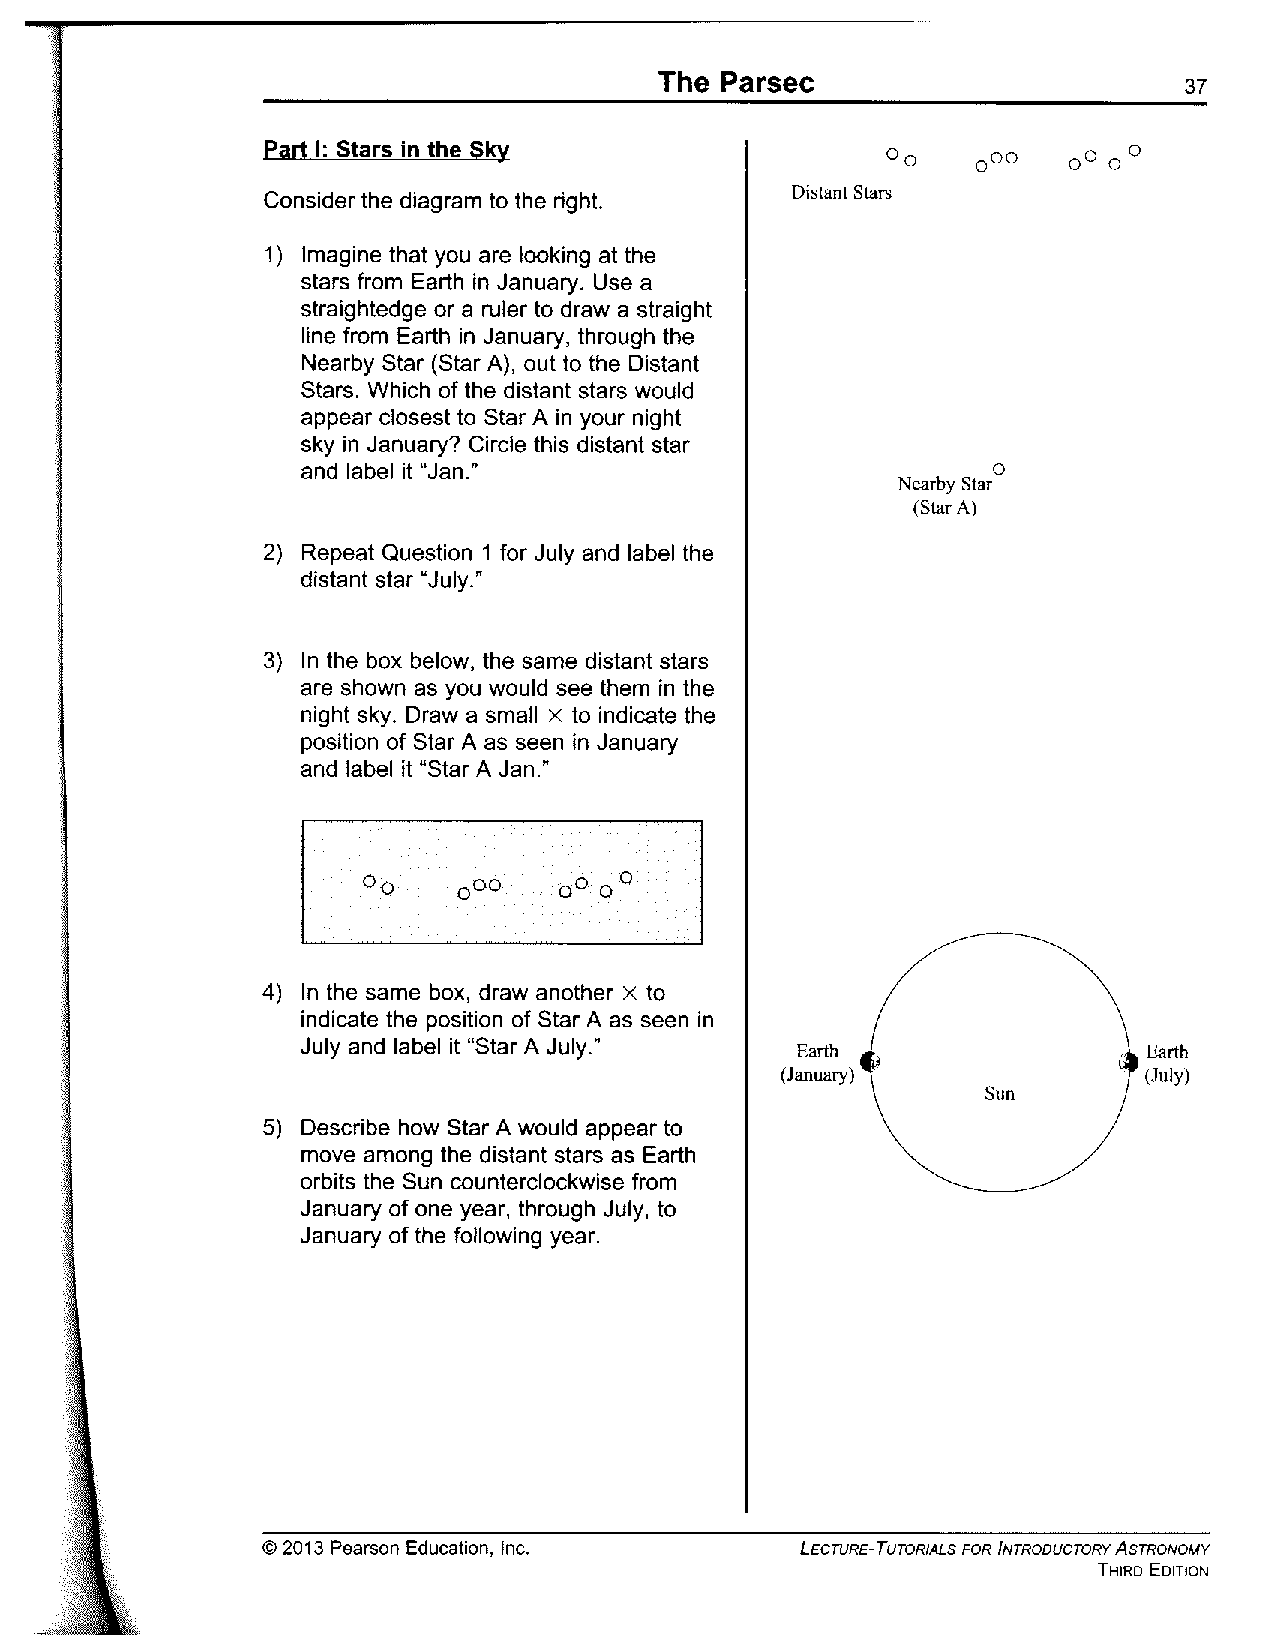
\includepdf[pages=1-3]{parallax/out.pdf}

\section{A quick measurement with hand tools}

You will now use the parallax technique to measure the distance to an object in your environment without needed to travel to it.

\begin{steps}
	\item Identify an object to be your ``nearby star'' and another as your ``distant star'', by analogy to the figure in the worksheet. Also choose the positions to view from as ``Earth (January)'' and ``Earth (July)''. When picking the stars and your Earth positions, check to see that from each Earth position, the distant star does not appear to move much, compared to the nearby star, and your guessed distance to the nearby star is at least 10 times greater than the distance between your two Earth positions.
\end{steps}
	
You'll first use crude measuring tools to compute the nearby star's distance with the parallax technique, and then use a more precise method. First, you'll use the little finger on your outstretched arm as a measurement of angular size --- the width of the index finger covers (``subtends'') about 1 degree.

\begin{steps}
	\item Identify an object to be your ``nearby star'' and another as your ``distant star'', by analogy to the figure in the worksheet. Find a place where you can stand and move a meter or two side to side and still see both ``stars''. The movement will simulate the Earth moving from its January to its July position. When picking the stars and your Earth positions, check to see that from each Earth position, the distant star does not appear to move much, compared to the nearby star, and your guessed distance to the nearby star is at least 10 times greater than the distance between your two Earth positions.
	
	\item Looking from just one eye, move so that the two stars appear to be just touching each other. Mark your current position as Earth (January). Hold up your smallest finger at arm's length and move to your left or right until your finger fits just in between the two stars. This means that they are 1 degree away from each other in angular separation. Mark this position as Earth (July).
	
	\item Draw a diagram, similar to the second figure in the worksheet, and find your own Earth-Sun distance (half the distance between your Earth positions). Calculate the parallax angle in radians, which is half the 1 degree you measured with your finger. For the distance measurement, you can use a ruler, measuring tape, or objects that have standard lengths like coins, paper money, or sheets of paper.
\end{steps}
	
Now the distance to the nearby star can be found using the triangle formed by the line segments Sun-Earth, Earth-Star, and Star-Sun (see Figure~\ref{par:fig:figure}). Trigonometry relates these lengths to each other according to
\begin{equation}
	\tan p = \frac{a}{d}\,,
\end{equation}
where $p$ is the parallax angle in radians, $d$ is the distance to the star, and $a$ is half of the distance between the two measurement positions. Since the length $d$ is much greater than $a$, the angle $p$ is very small, and so we can use the small angle approximation $\tan u \approx u$, and therefore
\begin{equation}
	p = \frac{a}{d}\,.
\end{equation}

\begin{figure}
	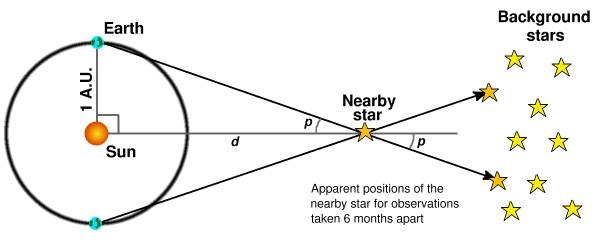
\includegraphics[width=\textwidth]{parallax/parallax-figure}
	\caption{Illustration of the geometry involved in a parallax measurement to determine $d$, the distance to a nearby star.}\label{par:fig:figure}
\end{figure}

\begin{steps}
	\item Use the above equation to calculate the distance to the nearby star.
	
	\item Conduct the data collection twice more to get two more Earth-Star distances. You can use this to calculate an uncertainty for your measurement --- the uncertainty is half the range of values, and the distance is the average of the 3 distances you found.
	
	\item Find the distance to the nearby star in a more direct way --- measure the distance with a measuring tape or pieces of paper, or for more distant objects, find them on Google Maps.
\end{steps}

One way of describing how different two values are, without considering the uncertainty of those values, is to calculate the percent difference:
\begin{equation}
\textrm{percent difference} = \frac{d_1 - d_2}{\left(\frac{d_1+d_2}{2}\right)} \times 100\%
\end{equation}

\begin{steps}	
	\item How close is your parallax distance measurement to the direct measurement? Report the percent difference.
\end{steps}
%Go out into the third floor hallway of KPTC (the long corridor near room 311).
%Go to the fifth floor of Eckhardt Research Center. Near the elevators on the north side, there are
%two telescopes%
% at the near end of the hallway, and an observing target is located at the far end.
%The target is a mock-up of the night sky, but with colors and relative sizes of objects greatly exaggerated to facilitate observations.

\section{Measuring with more precise equipment}

Using a finger for measuring angular separation is not very precise. Here you'll use the parallax technique to determine the same distance to the nearby star, but using a camera and analysis software instead.

%You will now use the telescope apparatus to measure the parallax of a “foreground star”
%(actually a ball on a stick)
%(actually a nearby building), with the
%mock-up star field
%Chicago skyline
%serving as “background stars.”
%Place the “foreground star” part way down the hallway between the telescopes and the observing target.
\begin{steps}
	\item Take a picture from a digital camera (likely your phone camera) from the vantage point of each Earth position used above.
	
	
%Make sure that it is positioned so that sightlines from both telescopes
%pass through both the “foreground star” and the “background stars,”
%(an overlapping background of the skyline).
%With your smartphone, take an image of the “foreground” and “background” stars through each telescope.
%Also measure the distance between the two telescopes using a measuring tape and record
%this value in your lab notebook. See Figure~\ref{par:fig:images} for example data.

%\begin{figure}
%	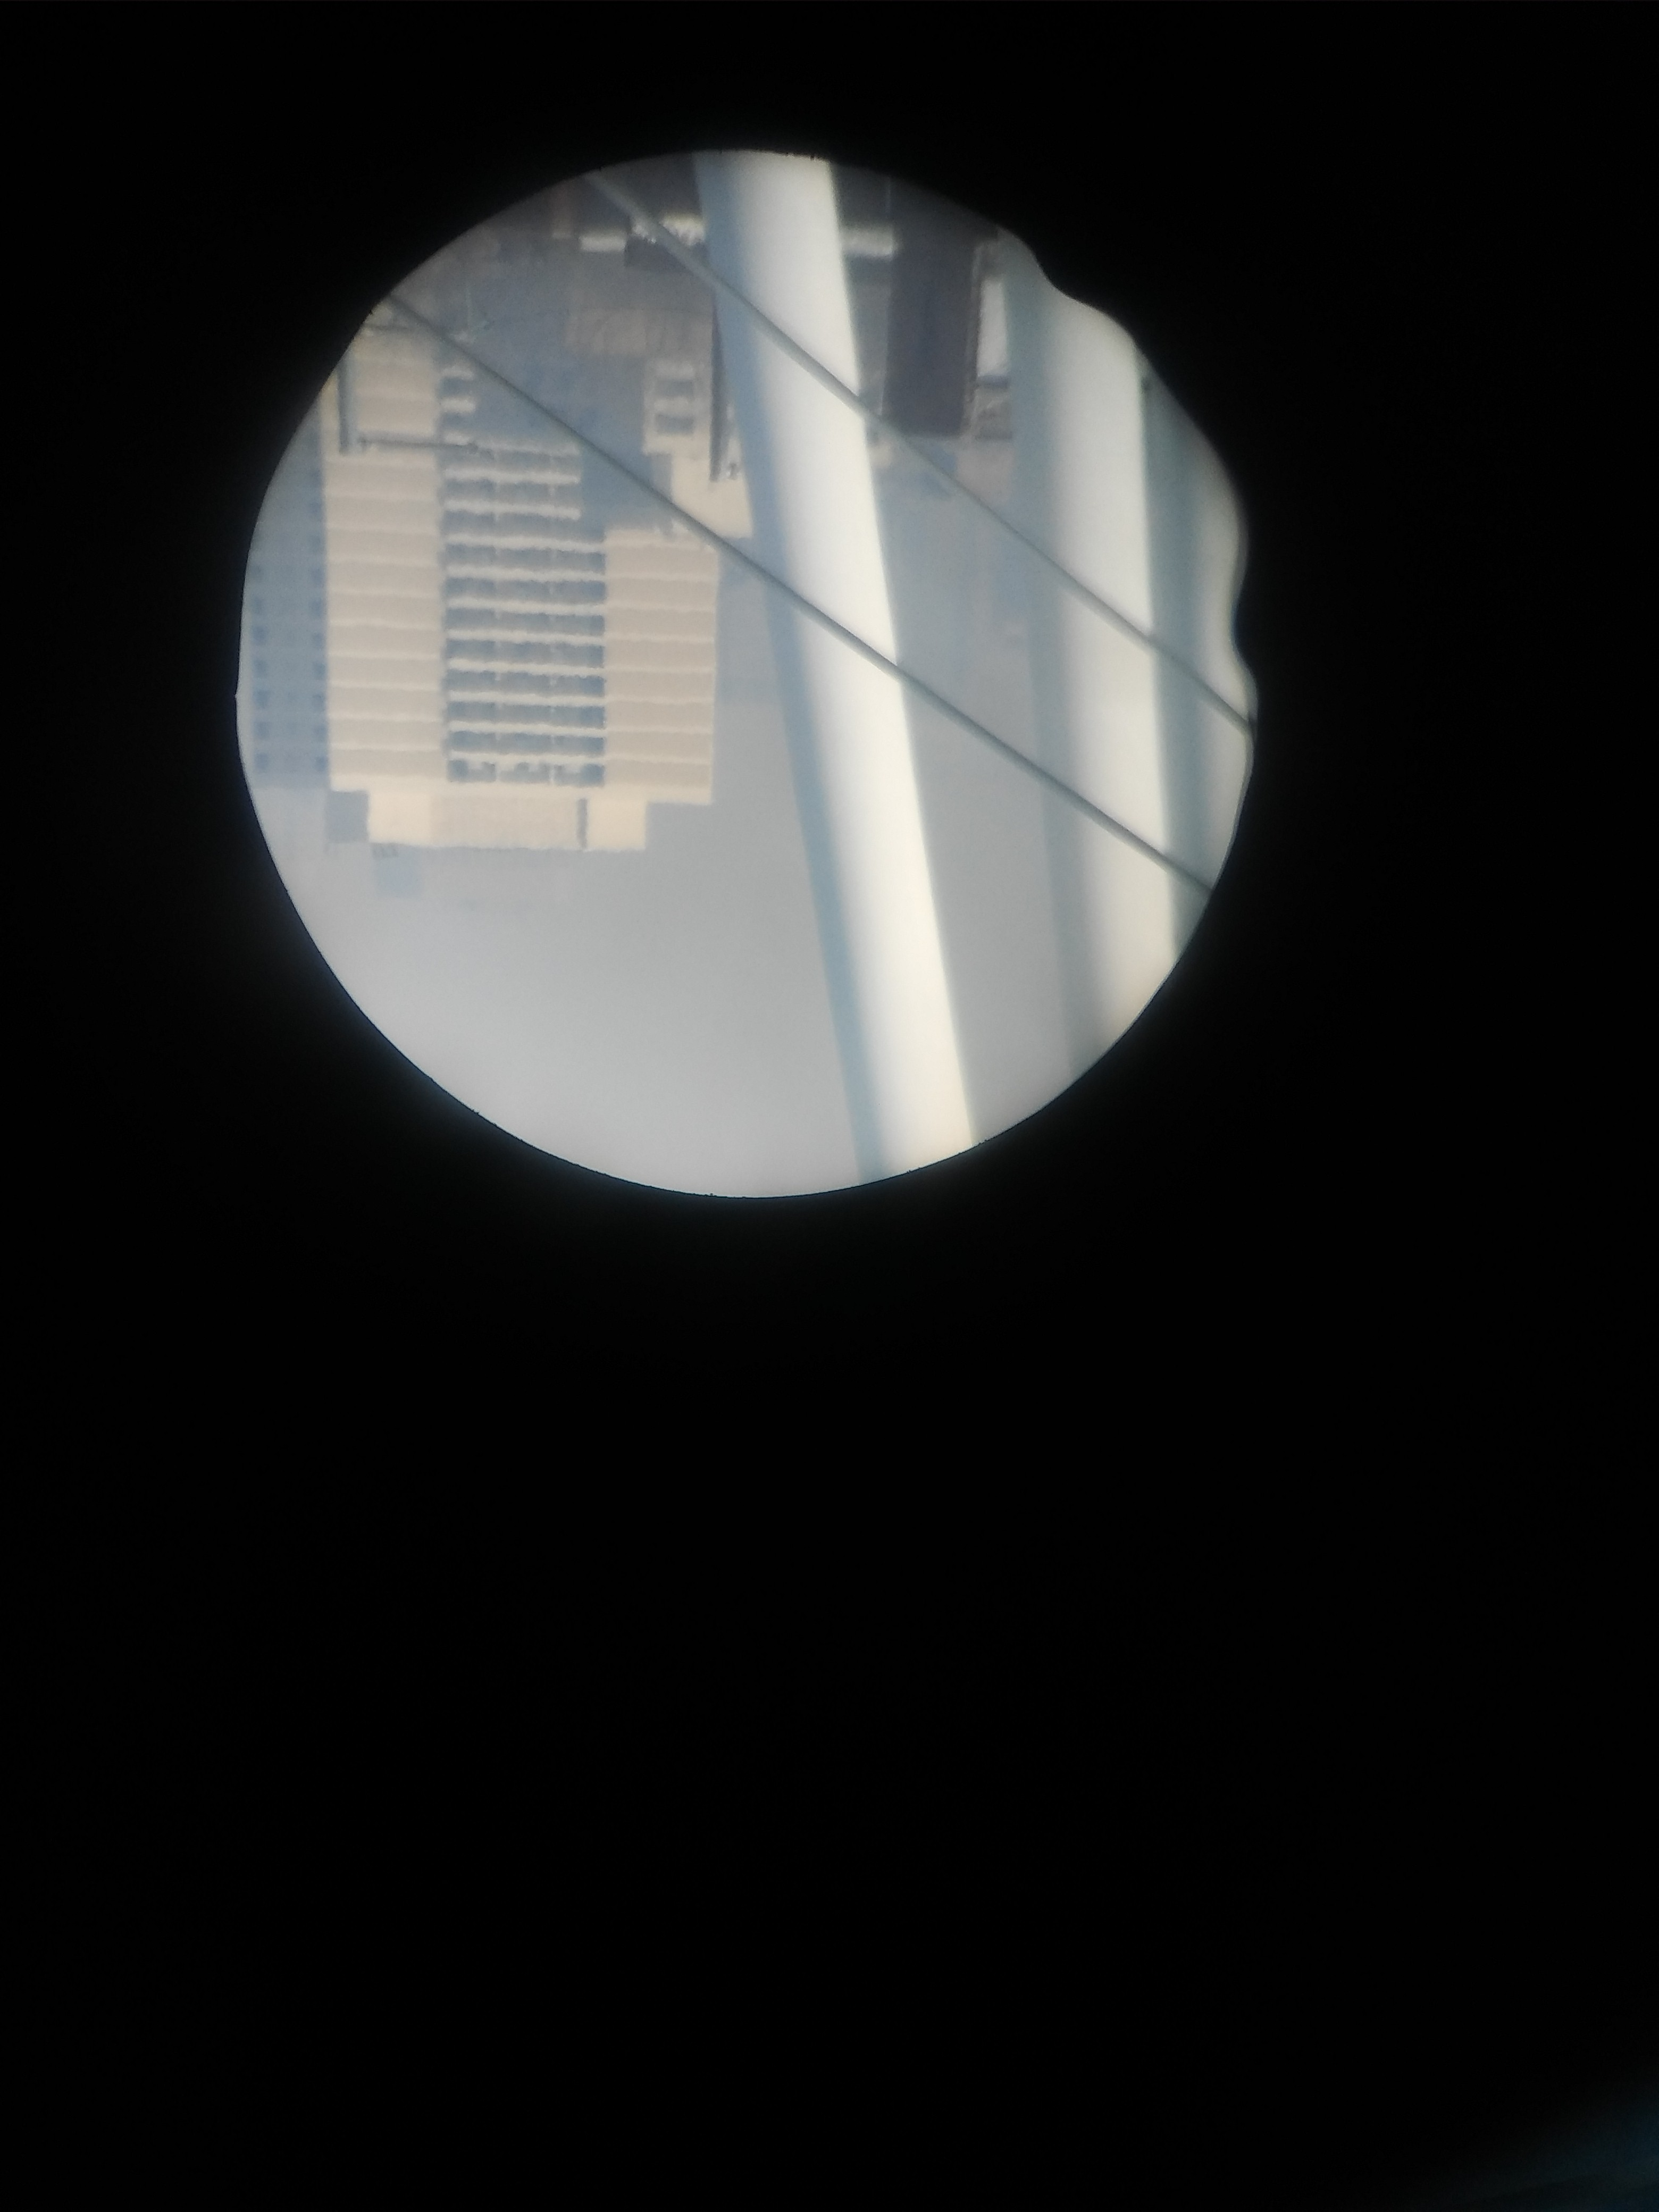
\includegraphics[width=0.5\textwidth]{parallax/parallax-image-1}
%	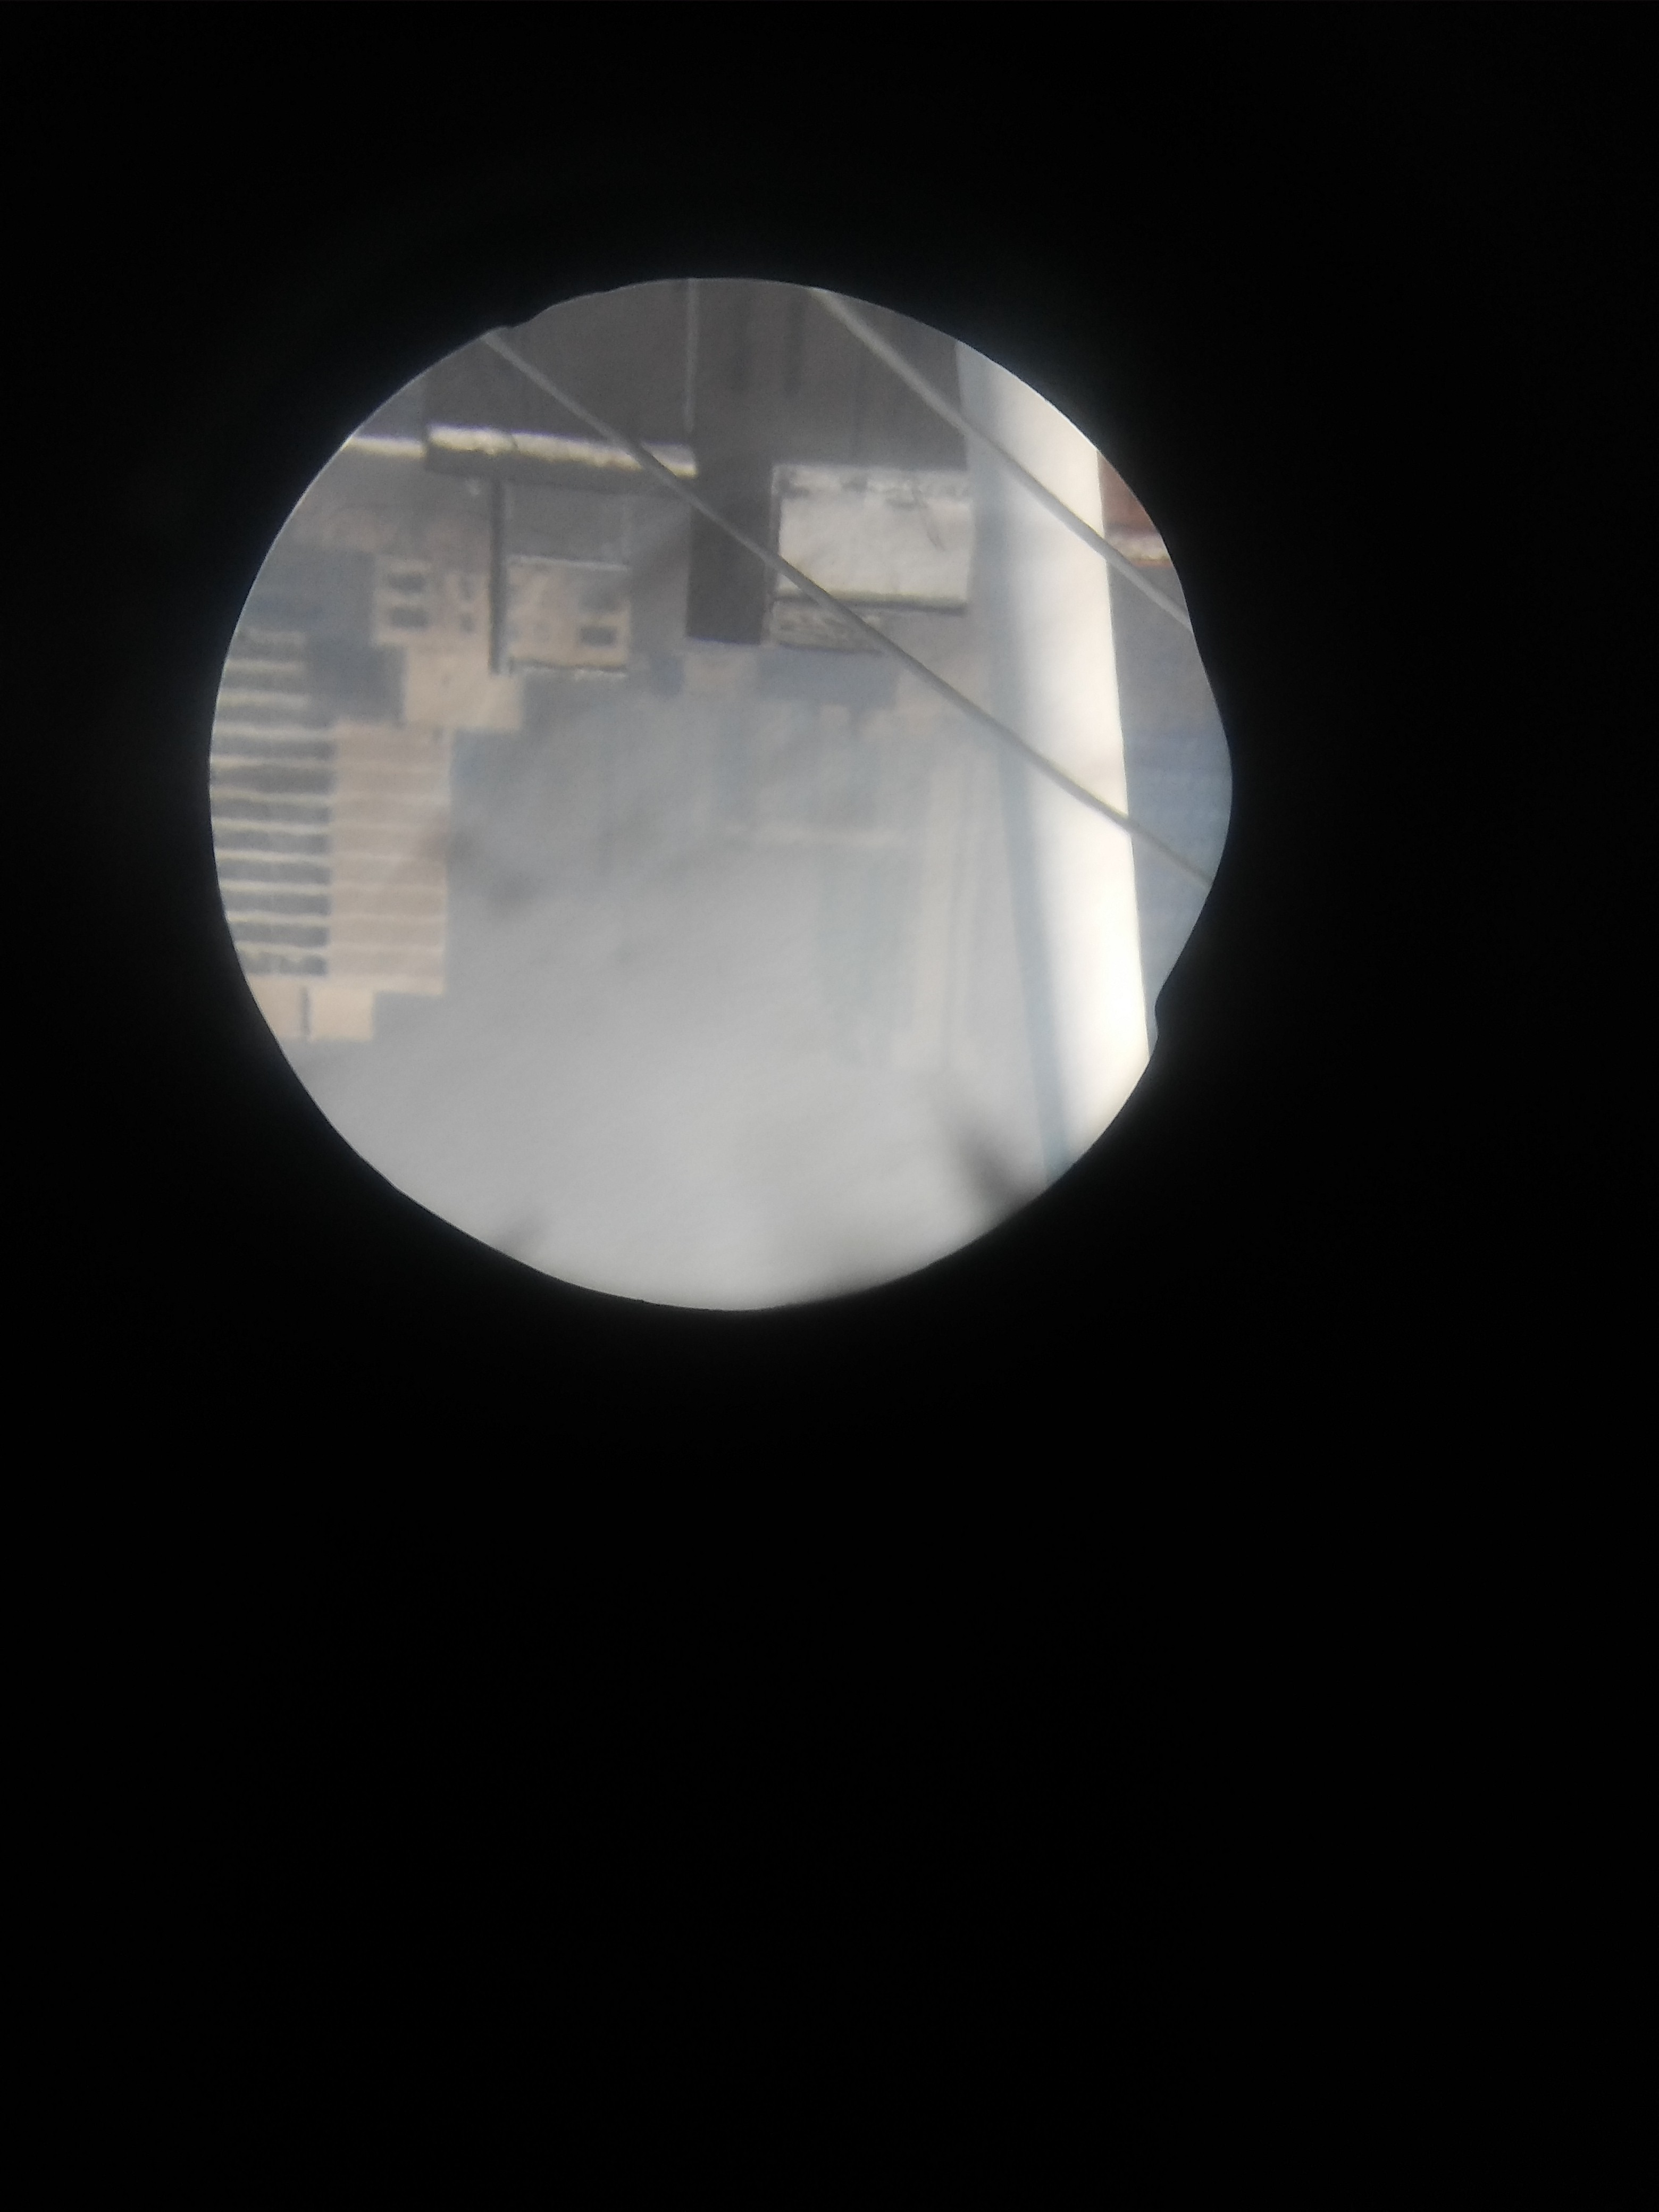
\includegraphics[width=0.5\textwidth]{parallax/parallax-image-2}
%	\caption{Example images. My foreground ``star'' was the point defined by the left intersection of the lower cable and the white pillar on top of the gym on campus. One of my reference ``stars'' was the top right corner of the building in the background. Note that the images produced by this telescope are upside down.}\label{par:fig:images}
%\end{figure}

%You have now finished collecting data, so now it’s time to analyze it. 
	\item Upload your photographs to a computer. The simplest way to do this may be to email the images to yourself from your phone. Give each file a descriptive name (e.g. ``\texttt{parallax\_left\_telescope}'').
\end{steps}

\subsection{Finding the pixel scale}

Notice that with the finger, I told you that your little finger, outstretched, is about 1 degree wide. This was a conversion between the linear size of your finger, for example 1 cm, to an angular size, 1 degree. With the camera, we need to find out the similar conversion --- how many pixels in an image corresponds to what angular size, also known as the \textit{pixel scale} of the image. To do this, you can take a known angular size and measure its length in pixels.
\begin{steps}
	\item Find an object of known length and place it a known distance from the camera (distance to camera should be 10 times or more the length of the object). Take a picture of that object.
\end{steps}

You will now convert the images from their default format (likely .png or .jpeg) into .fits
files, a format commonly used by astronomers. This format will be readable by SAO
Image DS9, an astronomical image analysis tool.
\begin{steps}
	\item Convert the image files to a .fits format using your favorite image processing software, or the software ``GIMP'' (Gnu Image Manipulation Program), or an image conversion website like \url{https://www.files-conversion.com/image/fits}. For using GIMP, open the file. From the FILE menu, select EXPORT AS, change the
file extension to “.fits,” and then click EXPORT. Repeat this procedure for each of your
images.

\item Open a saved .fits image of the pixel scale image in DS9. Your first task is to measure the pixel scale.
%Adjust the contrast so you can clearly see the field of view.
From the menu at the top of the screen, select REGION, SHAPE, LINE. On the first row
of buttons in the DS9 window, click EDIT then on the second row click REGION. Draw
a line along the known length of the object. On the first row of buttons, click REGION then on the
second row click INFORMATION. A window should pop up that will give you the length
of the line in physical units, that is, in pixels. \textbf{Record this value in your lab notebook.}

\item Find the angular size of the known object. Since the object is far away, we can again use the small angle approximation for the triangle involved and find that the angular size of the object is equal to its length divided by the distance to the object. This angle is in radians.

\item Find the pixel scale by dividing the number of pixels in the length by the angular size of the known object. This gives the pixel scale in pixels per radian.

\end{steps}
\subsection{Finding the parallax angle}

Now that you have the pixel scale of the image, you can use that to measure the parallax angle of the your nearby star and thus find the distance to that object like you did with the little finger method.

\begin{steps}
	\item Open the first parallax image. Measure the displacement from the nearby star to the distant star. Convert that displacement to radians using the pixel scale. Make sure to record both the X- and Y- offsets. Repeat these measurements for the second parallax image using the same distant star.

	\item Find the total angular distance the star moved between images. To do this, subtract the X- offsets from each other, and subtract the Y- offsets from each other. Then use the Pythagorean theorem to find the total distance moved ($d = \sqrt{x^2 + y^2}$). Divide this by two to get the parallax angle.
	
	\item Use Equation 2.2 to find your new calculation for the distance to the nearby star.
	
	\item Calculate the percent difference between this and the direct measurement like you did in the previous section.
\end{steps}

%Given that the field of view of the Galileoscope is 1.5\textdegree
% (0.75\textdegree with the Barlow eyepiece)
%calculate the \textit{plate scale} of your images, in arcsec/pixel.

%Select a reference star from your parallax measurements. Using your plate scale,
%determine the angular separation between the reference star and the target star. Record
%the value for the total separation, $r$, and for both the horizontal ($x$) and vertical ($y$) components. You can
%check your measurements against each other by inputting these values into the
%Pythagorean formula: $r^2 = x^2 + y^2$. Do your measurements agree?
%
%Repeat the above calculations for all reference stars in both of your parallax images. You
%can now calculate the distance to the foreground star. The distance to a star can be found using the triangle formed by the line segments Sun-Earth, Earth-Star, and Star-Sun (see Figure~\ref{par:fig:figure}). Trigonometry relates these lengths to each other according to
%\begin{equation}
% \tan p = \frac{a}{d},
%\end{equation}
%where $p$ is the parallax angle in radians, $d$ is the distance to the star, and $a$ is half of the distance between the two measurement positions. Since the length $d$ is much greater than $a$, the angle $p$ is very small, and so we can use the small angle approximation $\tan u \approx u$, and therefore
%\begin{equation}
%p = \frac{a}{d},
%\end{equation}



%Use each reference star to calculate an independent measurement of parallax. To do this, for each reference star, you'll need to find how far (in radians) the target star has moved between the two observations. Using vector arithmetic\footnote{See \url{https://www.mathsisfun.com/algebra/vectors.html} for a short tutorial}, subtract the two displacement vectors from each other by components and find the magnitude of that difference vector. Divide by 2 and convert to radians to find $p$. After finding $p$ from each reference star, average these values together and estimate your uncertainty by finding the standard deviation of these measurements. You can perform this calculations in Excel using the functions AVERAGE() and STDEV(). Report your measurements in a table in your lab
%report.
%
%Also use a map to find the distance from you to your foreground star (with uncertainty). Compare these quantities with their uncertainties using the procedure found in Appendix~\ref{unc:sec:comparing}, to see the degree to which they agree.

\section{Questions}\label{par:sec:questions}

These should be included in your lab report.

\begin{steps}
	\item Your parallax measurements depend on an incorrect implicit assumption. What is
	this assumption, and how will it bias your results? How would you change the
	procedure in order to minimize this bias?
	\item What were the primary sources
	of uncertainty? How would you improve the procedure for future measurements?
\end{steps}

\section{Report checklist}

Include the following in your lab report. See Appendix~\ref{cha:lab-report-format} for formatting details. Each item below is worth 10 points.

\begin{enumerate}
	\item The completed worksheet ``The Parsec''.
	\item Work and final answer for your distance measurements using your finger, with uncertainty.
	\item Work and final answer for direct distance measurement, along with percent difference.
	\item A figure with your three images (pixel scale image and two parallax images).
	\item The displacement vectors from distant star to nearby star.
	\item Final determined value of the distance and comparison with the direct distance. Show your work (see Appendix~\ref{cha:lab-report-format}).
	\item Answers to the questions in Section~\ref{par:sec:questions}, with justification.
	\item A 100--200 word reflection on group dynamics and feedback on the lab manual. Address the following topics: who did what in the lab, how did you work together, what successes and challenges in group functioning did you have, and what would you keep and change about the lab write-up?
\end{enumerate}
%\chapter{Measuring the distance to a galaxy using globular clusters}

%todo add lab activity to measure differential light intensity at different distances from light bulbs
%todo clarify that M5 (rather than Sun) should be used to compare to M87 cluster
%todo describe M classification system, that they can represent different kinds of things

%In this lab, you will measure the distance to the Virgo galaxy, which we will use for next week’s laboratory as the first rung in our distance ladder measuring the distance to other galaxies.

In this lab, we will use a globular cluster in the Milky Way called M5 (see Figure~\ref{gc:fig:m5}) as the first step of our distance
ladder to other galaxies. By comparing this globular cluster to another in a nearby galaxy
called M87 in the Virgo cluster, we will estimate its distance, adding another rung to our
distance ladder. Ideally, we should compare many globular clusters in the Milky Way to
M87, here we will use just one cluster, which is enough to demonstrate the principle.

\begin{figure}
	\centering
	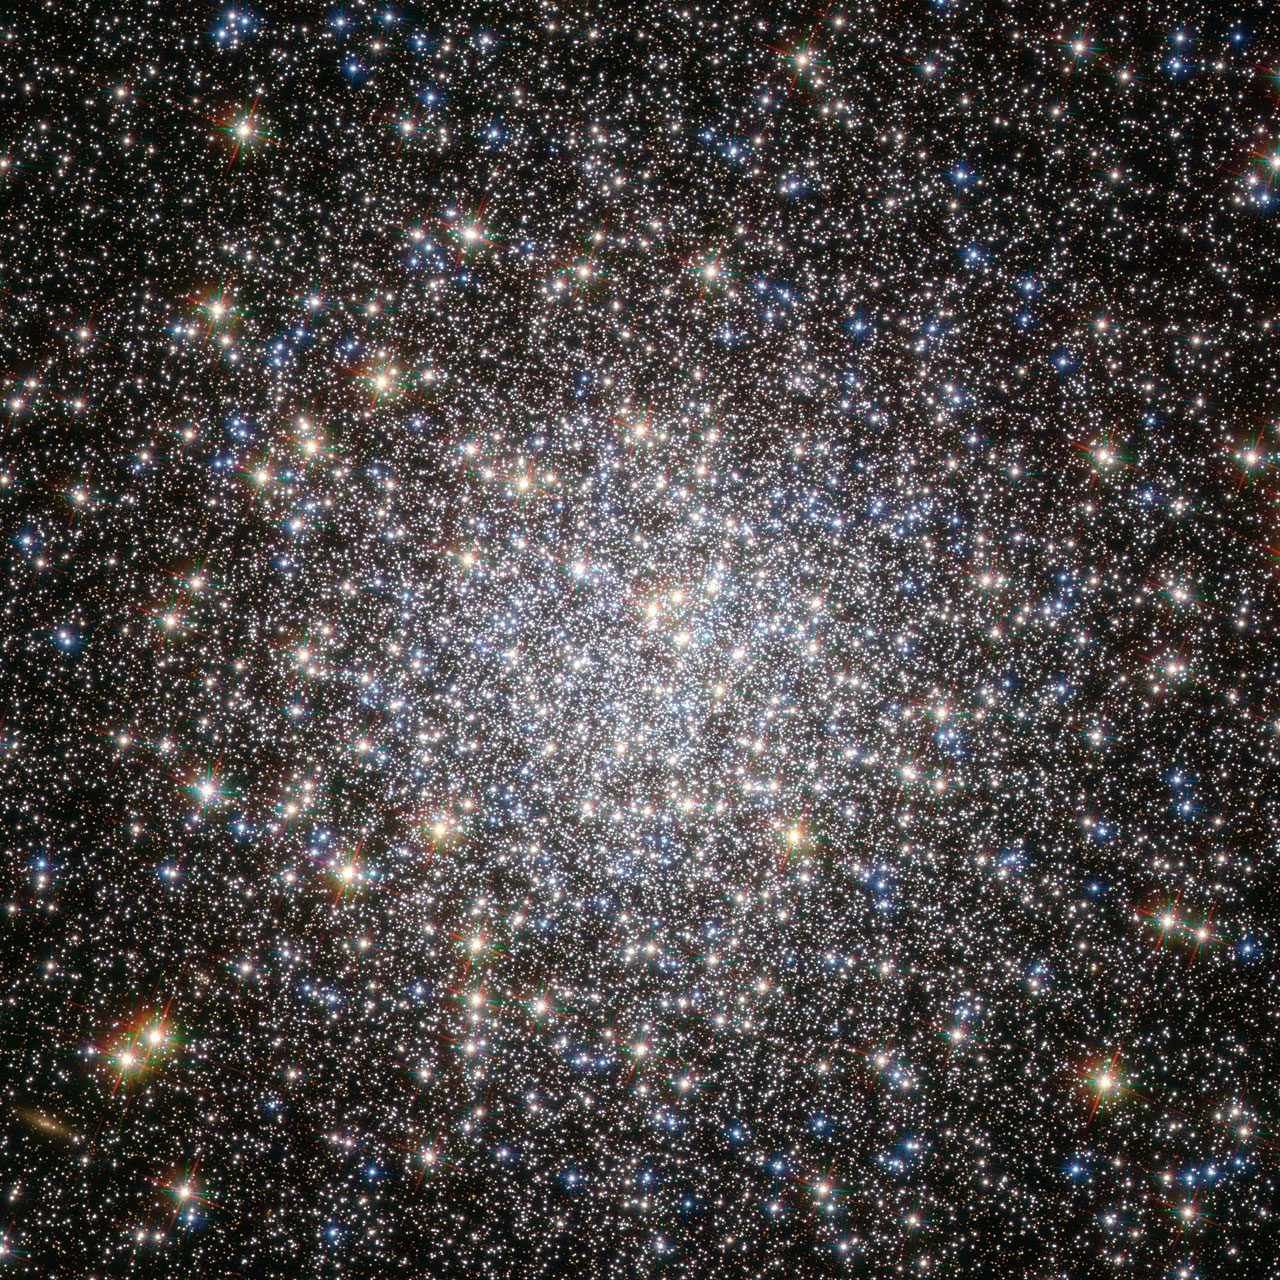
\includegraphics[width=0.7\textwidth]{globular-cluster/potw1118a}
	\caption{Messier 5 (M5) is a globular cluster (a gravitationally bound collection
		of stars) of more than 100,000 stars in the Milky Way Galaxy. Located at Right
		Ascension (RA) = 229.640\textdegree, and Declination (Dec) = 2.075\textdegree.
		The above
		image is 2.85 arcmin on a side, or about 1/20th of a degree.
		Image source: ESA/Hubble \& NASA, \url{http://www.spacetelescope.org/images/potw1118a/}}\label{gc:fig:m5}
\end{figure}

If two identical lightbulbs are placed with one close to you and another farther away, the more distant one will appear dimmer. This is because the light from a spherical emitting source spreads out over a spherical shell that gets larger as the light gets more distant from the source. So if sources 1 and 2 have the same luminosity, then their distances $d$ and apparent brightness
$b$ are related by
\begin{equation}
\frac{b_1}{b_2} = \left( \frac{d_2}{d_1} \right)^2 \,.
\end{equation}
Since the numbers we will extract from the images are either in brightness or magnitudes,
it is convenient to re-cast this relation in terms of magnitudes. Magnitudes $m_1$ and $m_2$ are
related to brightness $b_1$ and $b_2$ by
\begin{equation}
m_2 - m_1 = 2.5 \log \left[ \left( \frac{b_1}{b_2} \right)^2 \right] \,.
\end{equation}
Combining the two equations, we get
\begin{equation}\label{gc:eq:m-d}
 \log(d_1/d_2) = 0.2 (m_1-m_2) \,.
\end{equation}
This says that once we have measured magnitudes $m_1$ and $m_2$ for two sources, then we can
derive the ratio of their distances from us, \textit{as long as they have the same luminosity}.

\section{Road Map}

To keep track of the steps in this lab, we will fill in Table~\ref{gc:tab:mag}. In this table, the entry for the magnitude of M5 refers to the sum of all of its stars. In
principle, we could measure this ourselves with the roof-top telescope, but for this lab we take
a value from a catalog of such data. The SDSS data cannot be used because the stars
are too crowded together for an accurate measurement.

\begin{table}
	\centering
	\begin{tabular}{l|c|c}
		\toprule
		\textbf{Object} & \textbf{Magnitude} & \textbf{Distance (AU)} \\ \midrule
		Sun & -26.89 & 1 \\\midrule
		Sun-like stars in M5 &  & \\\midrule
		M5 itself & 5.65 & \\\midrule
		M87 globular clusters & &
		\\ \bottomrule
	\end{tabular}
	\caption{Table of magnitude and distance.}\label{gc:tab:mag}
\end{table}

The first step is to make a \textit{color-magnitude diagram} for the stars in M5 to find a star that
has similar to the Sun; we assume that such a star has the same luminosity as the Sun. The
magnitude of the star (specifically its $r$-band magnitude) gets entered into the above table,
and you derive the distance to M5.

The second step is to identify faint things surrounding the galaxy M87 that are likely to be
globular clusters associated with it, and get their magnitudes (again the $r$-band magnitude)
from the database. Some value that properly represents the ensemble gets entered into the
above table and you derive the distance to M87 by comparing the magnitudes of M5 and M87.

\textit{To summarize:} the distance to the Virgo cluster depends on two assumptions: 1) stars
with Sun-like colors in the globular cluster M5 have the same luminosity of the Sun. 2)
Globular clusters like M5 in the Milky Way have luminosities that are comparable to
the globular clusters in M87. Neither of these assumptions is necessarily well justified based on information available to you, but there are checks that reassure us that the assumptions
are good enough for at least a first estimate of distance.

\section{Analyzing the M5 globular cluster}

First you'll retrieve from an online database the magnitude of stars in the region of sky where M5 is. In the window at \url{http://skyserver.sdss.org/dr13/en/tools/search/sql.aspx}, enter the following query:

\begin{verbatim}
SELECT TOP 200
   objid,ra,dec,u,g,r,i,z
FROM Star
WHERE
   r BETWEEN 10 AND 23
   AND ra between 229.50 and 229.78
   AND dec between 2.2 and 2.3
\end{verbatim}

\subsection{Questions and results for your report}

\begin{steps}
	\item From the data above, create a .csv file, rename it M5.csv. Read it into
	a spreadsheet, and make columns for the colors $g - r$, $r - i$, and $g - i$. The Sun has
	colors $g - r = 0.44$, $r - i = 0.11$, and $g - i = 0.55$. Plot the $r$ magnitude vs. one of the colors (e.g.
	$g - r$), and reverse the $r$ magnitude axis, since lower magnitudes represent brighter objects. On this color-magnitude diagram, identify
	the \textit{main sequence} of stars. This plot is called a color-magnitude diagram, which is similar to an H-R diagram as seen in Figure~\ref{gc:fig:hr}.
\end{steps}

\begin{figure}
	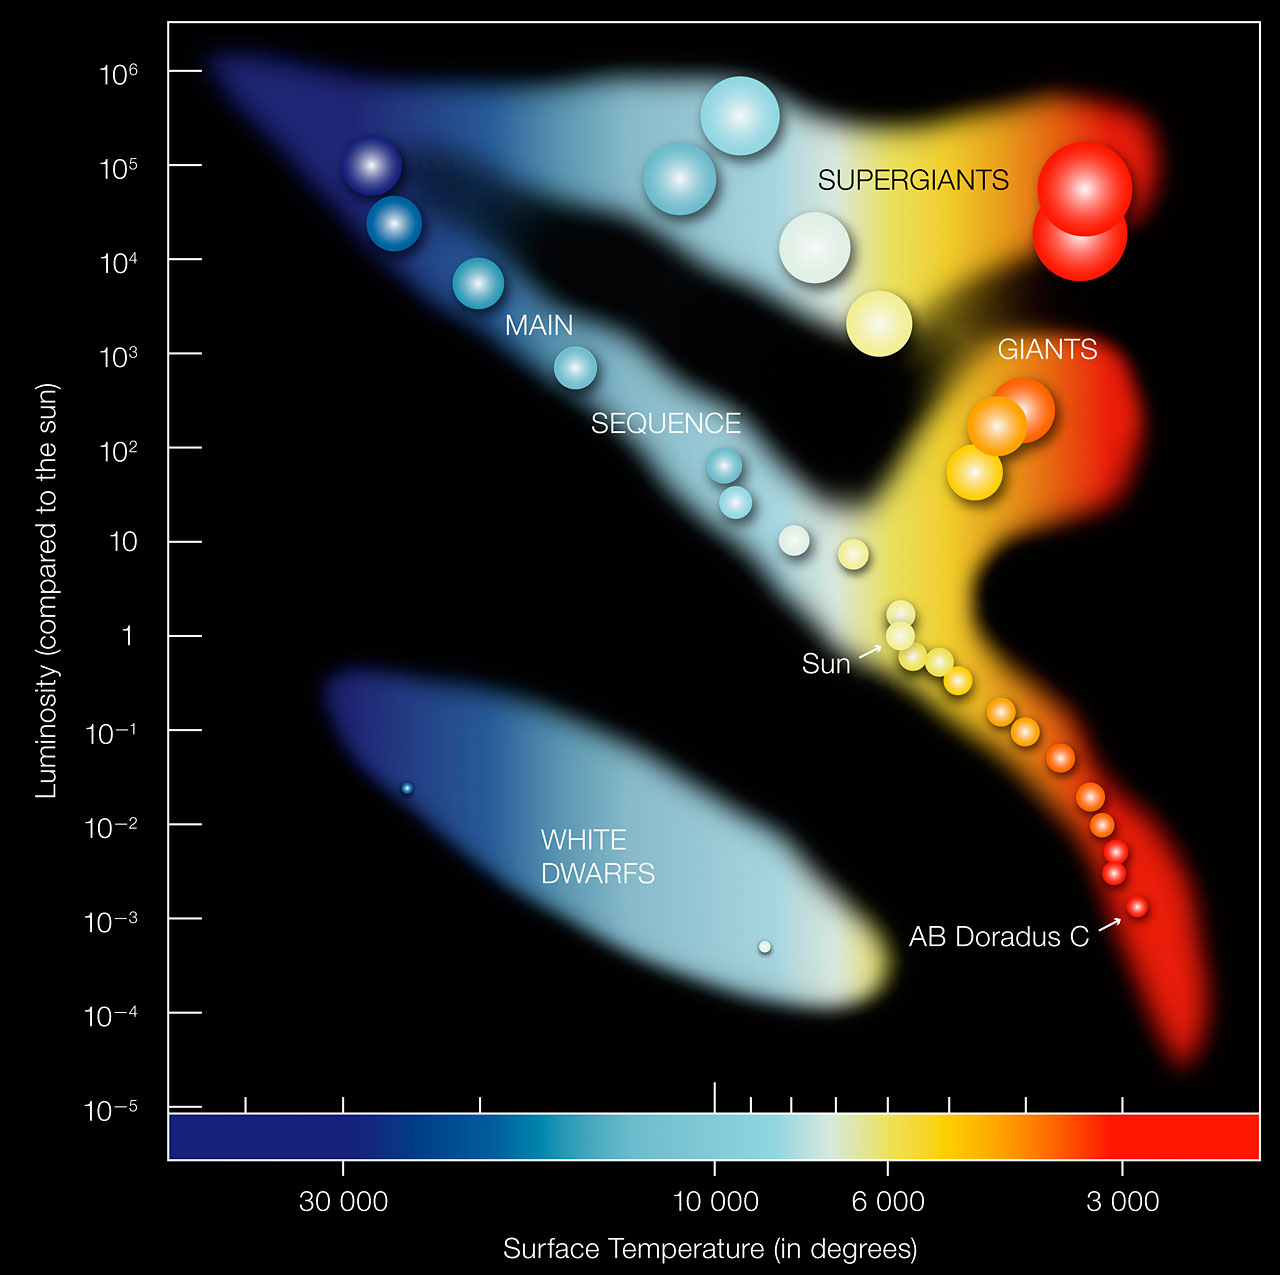
\includegraphics[width=\textwidth]{globular-cluster/eso0728c}
	\caption{Herzsprung-Russell (H-R) diagram, plotting stars according to their luminosity and surface temperature. Luminosity is related to magnitude, and surface temperature is related to color. Image Source: ESO (\url{https://www.eso.org/public/images/eso0728c/}}\label{gc:fig:hr}
\end{figure}

\begin{steps}
	\item Begin to fill out Table~\ref{gc:tab:mag} with the magnitude and distance to a Sun-like star
	in M5. When you finish this lab and turn in this lab report, this table will
	be completely filled out.
\end{steps}

\section{Analyzing the globular clusters near the M87 galaxy}

Figure~\ref{gc:fig:m87} shows the field surrounding the giant Virgo galaxy M87, also known as NGC 4486.

\begin{figure}
	\centering
	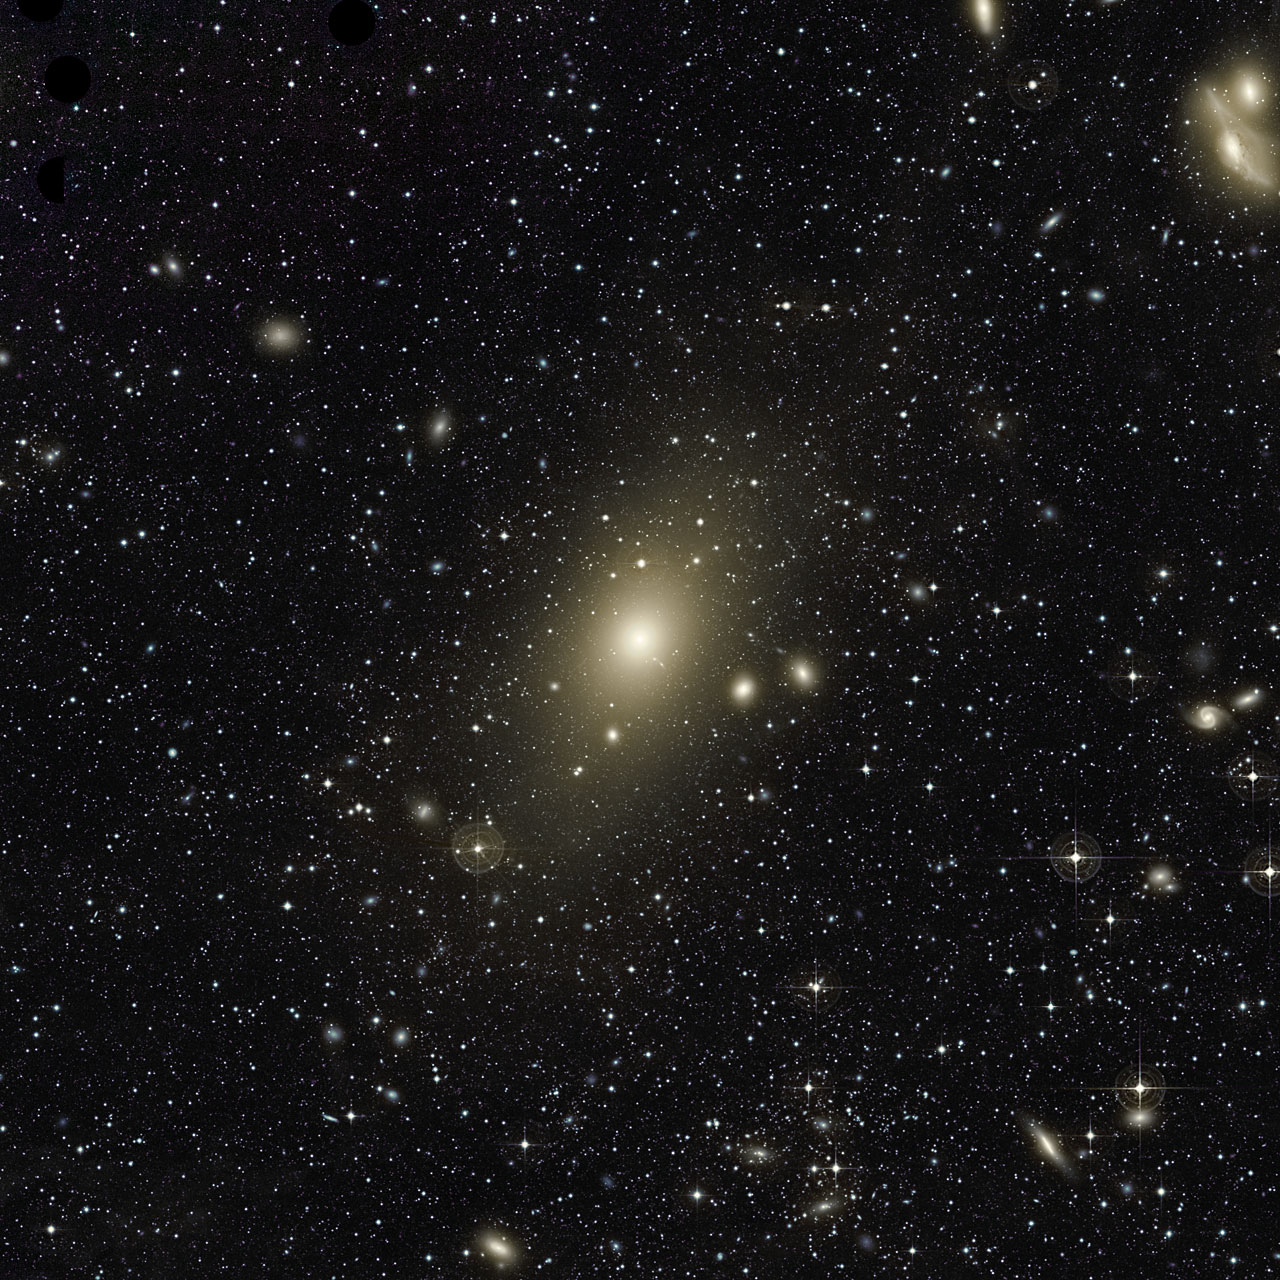
\includegraphics[width=0.7\textwidth]{globular-cluster/eso1525a}
	\caption{Messier 87 (M87) is a nearby elliptical galaxy in the constellation Virgo. It is
		known for having a large population ($\sim 10,000$) of globular clusters, about 100 times more
		than the Milky Way Galaxy. Centered at RA=187.706\textdegree and Dec=12.391\textdegree, the above image
		is 97 arcminutes across. Image source: Chris Mihos (Case Western Reserve University)/ESO, \url{http://www.eso.org/public/images/eso1525a/}.}\label{gc:fig:m87}
\end{figure}

The task is to find the magnitudes for the faint speckles surrounding M87 that are barely visible in
Figure~\ref{gc:fig:m87}, namely its globular clusters. We set up a similar query to that used for M5, except
of course the coordinates (RA, Dec) are different. Enter the following query:

\begin{verbatim}
SELECT TOP 200
   objid,ra,dec,u,g,r, i,z
FROM Star
WHERE
   r BETWEEN 10 AND 23
   AND ra between 187.591 and 187.821
   AND dec between 12.278 and 12.504
\end{verbatim}

The globular clusters are so far away that each cluster of stars appears as, and is categorized as, stars in
the SDSS database. As a cross-check, also run the above query in a random piece of sky at least
5\textdegree away.

\subsection{Questions and results for your report}

\begin{steps}
	\item Make color-magnitude diagrams for both samples (M87 and random-sky)
	and compare them. Does either either color-magnitude diagram show any
	evidence for a correlation between brightness (magnitude) and color for the
	plotted points?
	
	\item Once you have identified which of the sources on your M87 color-magnitude
	diagram can be identified with a population of globular clusters surrounding
	M87, argue which apparent magnitude should be selected to enter into the table, and do so. Why is there a range of magnitudes? How would you make this
	process more precise? What other sources of uncertainty do you think
	there are?
	
	\item Calculate the distance to M87 using Equation~\ref{gc:eq:m-d}, comparing its magnitude to that of M5. If you have not already converted AU to
	parsecs, do so now to get the distance in mega-parsecs ($1\:\mathrm{Mpc} = 2.06 \times
	10^{11}\:\mathrm{AU}$). The accepted value for the distance to the Virgo cluster is 16.4
	Mpc. From your uncertainties above, how well do these two values agree within your expected level
	of uncertainty? See Appendix~\ref{unc:sec:comparing} for details of how to determine this.
	
	\item Based on the distance you found, when did the light from the Virgo galaxy arrive at the sky survey's telescope? What was happening on Earth at that time?
\end{steps}

\section{Include in your report}

Each of the following items will be graded out of 10 points.

\begin{itemize}
	\item Completed table
	
	\item Three color magnitude graphs
	
	\item Questions 1--2 from the first section
	
	\item Questions 3--6 from the second section
	
	\item A 100--200 word reflection on group dynamics and feedback on the lab manual. Address the following topics: who did what in the lab, how did you work together, what successes and challenges in group functioning did you have, and what would you keep and change about the lab write-up?
		
\end{itemize}
%\chapter{Galactic distances and the Hubble diagram}

%todo remove a couple galaxies - some are especially difficult to see the Ca lines with.


\section{Introduction}

In 1929, Edwin Hubble measured that distant galaxies were
systematically redshifted relative to galaxies that were closer. From this
data, Hubble inferred that the universe was expanding, an idea initially
worked out by Georges Lemaitre using Einstein's theory of gravity.

In this lab, you will conduct a measurement similar to Hubble's and will
produce your own version of his famous Hubble diagram shown below.

\section{Building intuition}

The graph in Figure~\ref{hd:fig:hubble-diagram-schematic} illustrates the impact of an expanding universe of
photons emitted from distant objects. Because the speed of light is
constant, photons that we measure today were emitted in the past, with
photons originating from objects that are further away being emitted
earlier in time. This means that photons from objects that are further
away are older, and thus, those photons have experienced more expansion by the universe.

\begin{figure}
	\centering
	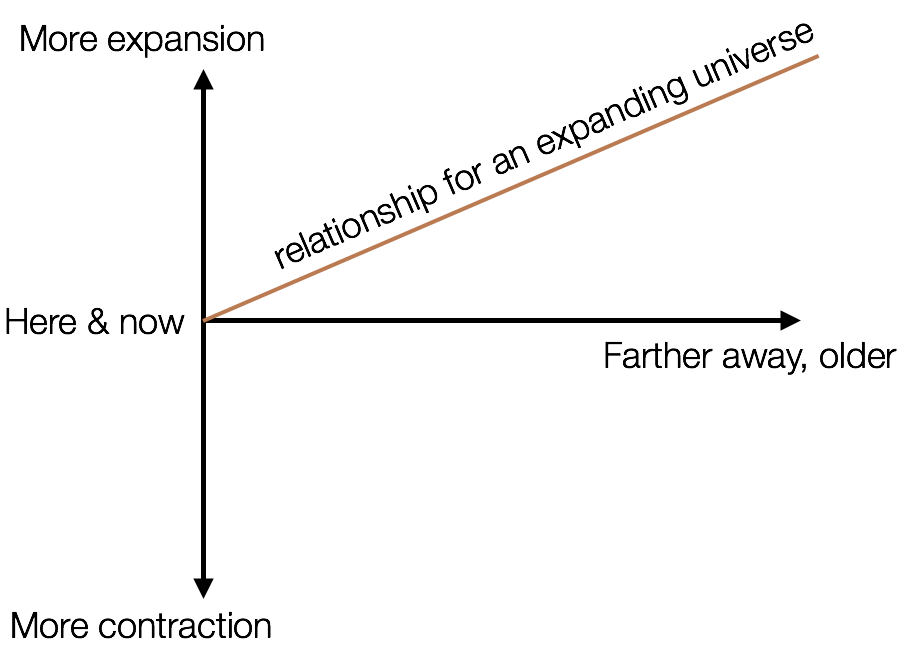
\includegraphics[width=0.5\textwidth]{hubble-diagram/hubble-diagram-schematic}
	\caption{Schematic of a Hubble diagram plot. It illustrates the relationship between the expansion
		experienced by a photon and the distance of its emitter.}\label{hd:fig:hubble-diagram-schematic}
\end{figure}

\begin{steps}
	\item\label{hd:step:sketch} Sketch the plot from Figure~\ref{hd:fig:hubble-diagram-schematic}, then sketch on the plot two more lines corresponding to the
	relationship for 1) a contracting universe, and 2) a static universe.
\end{steps}

From this relationship, we can determine whether the universe is
expanding, contracting, or static by looking at a number of galaxies and
measuring their distance (corresponding to the horizontal axis) and the
expansion experienced by their photons (corresponding to the vertical axis).

For this lab, we will use galaxy images and spectra listed in an online
table.

\section{Measuring distance}

We will use geometry to measure the distance of our galaxies. Galaxies
that are closer will look bigger and will subtend a larger angle whereas
galaxies that are further will looks smaller and will subtend a smaller
angle. This relationship between the angular size of the galaxy and its
distance is illustrated in Figure~\ref{hd:fig:galaxy-subtend}.

\begin{figure}
	\centering
	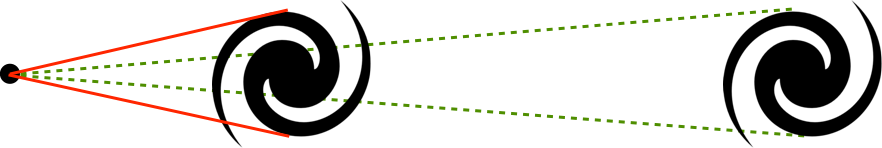
\includegraphics[width=\textwidth]{hubble-diagram/galaxy-subtend}
	\caption{Looking from the dot on the left, there are two galaxies that are the same size, one further away than the other. The more distant galaxy subtends a smaller angle (dashed green lines) than the closer galaxy (solid red lines).}\label{hd:fig:galaxy-subtend}
\end{figure}

Our galaxies will all be nearly the same size (22 kpc). Using the
geometry shown in the illustration, we can arrive at the following
relationship:
\begin{equation}\label{hd:eq:size}
 \textrm{angular size} = \frac{22\:\textrm{kpc}}{\textrm{distance}} \,.
\end{equation}
So, by measuring the angular size of our galaxy images, we can use the
above equation to determine the distance to the galaxy.

From the Files section of the Canvas site, download and extract to a folder \texttt{HubbleDataWebpage.zip}. In that folder, open \texttt{HubbleDataPage.html}. You
will find a list of galaxy names. Click on the ``Image'' link for the first
galaxy, NGC 1357. In the new tab, you will see an image of galaxy NGC
1357 similar to Figure~\ref{hd:fig:galaxy-example}.

\begin{figure}
	\centering
	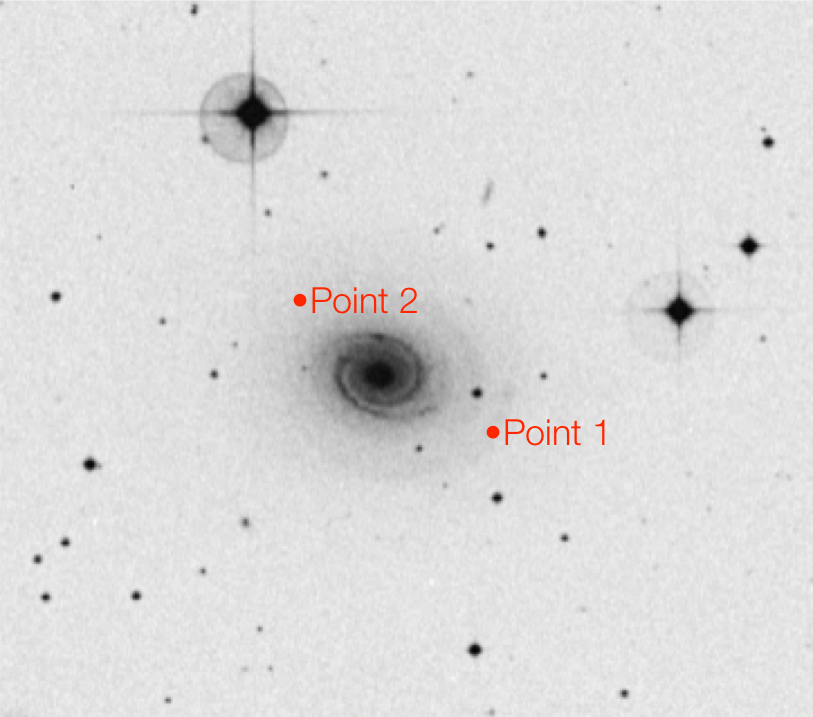
\includegraphics[width=0.5\textwidth]{hubble-diagram/galaxy-example}
	\caption{Example of galaxy image. Colors are inverted here, and Points 1 and 2 mark the furthest extent of the galaxy}\label{hd:fig:galaxy-example}
\end{figure}

\begin{steps}
	\item\label{hd:step:kind} What kind of galaxy is it (spiral, elliptical, unclear)? Note this in your spreadsheet.
	
	\item Are there any noteworthy features in the image? Use your spreadsheet to record your answers.
\end{steps}

We want to measure the angular size of NGC 1357, which you can do by
measuring the angular separation between two appropriate points
spanning the entire galaxy. In the lower left hand corner of google
skymaps, google shows you the coordinates of your cursor. Record the
coordinates (RA and DEC) for two points spanning the galaxy. Then use
an online calculator (e.g.
\url{http://cads.iiap.res.in/tools/angularSeparation}) to calculate the
angular separation between the points. Be careful and make sure that you don’t choose points that are too far
outside or inside the galaxy image.

\begin{steps}
	\item\label{hd:step:size} Enter the value for the angular size
(in radians, not degrees) in a spreadsheet.

	\item Divide up the remaining galaxy images between your groupmates
	and repeat Steps~\ref{hd:step:kind}--\ref{hd:step:size} for each of the galaxies recording your notes
	and measurements in the spreadsheet.
	
	\item Once you have measured the angular size of all the galaxies, use Equation~\ref{hd:eq:size} to estimate the distance for each galaxy
	and record the values in a “distance” column.
\end{steps}





\section{Measuring expansion}

The wavelength of light changes as the universe expands, an effect
known as cosmological redshifting. If the universe expands, the
wavelength is stretched, becoming longer and redder. For a contracting
universe, the wavelength will be compressed becoming bluer. We define
the redshift, $z$, as
\begin{equation}\label{hd:eq:redshift}
 z = \frac{\lambda_\textrm{measured} - \lambda_\textrm{original}}{\lambda_\textrm{original}} \,,
\end{equation}
where $\lambda$ represents the wavelength. The redshift is a measure of how much the wavelength has been
stretched or compressed.

We can measure the redshift by examining spectra (the energy emitted
in different wavelengths) of the same galaxies we just measured. For
NGC 1357, click on the link “Ca Spectra.” The link will show spectra
associated with Ca absorption which produces dips at wavelengths of
3933.7 Angstroms and 3958.5 Angstroms. You should see two
prominent dips in the data. See Figure~\ref{hd:fig:spectra} for example spectra.

\begin{figure}
	\centering
	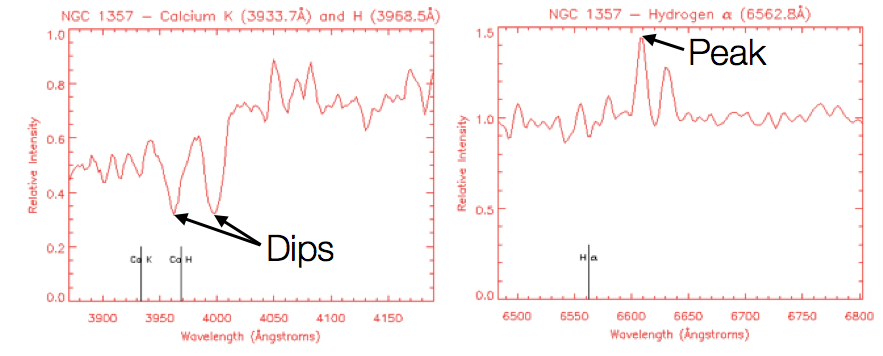
\includegraphics[width=\textwidth]{hubble-diagram/spectra}
	\caption{Spectrum of light detected from NGC 1357. The dips and peak that you will use to identify redshift are identified.}\label{hd:fig:spectra}
\end{figure}

Go back to the galaxy list and click on the
link “H-alpha spectrum” to bring up the spectra associated with
Hydrogen alpha emission of light with wavelength 6562.8 Angstroms.
You should see a clear peak in the data. The H-alpha peak is the leftmost
of the distribution. Since we know the original wavelengths for these
processes, we can compare the measured wavelength of these features
with their original wavelength to determine how much the light has
stretched.

\begin{steps}
	\item For each of the spectra estimate the value for the two Ca dips and the H-alpha peak. Record the values for the two Ca absorption lines and the H-alpha emission line in the excel worksheet. 
	
	\item Use Equation~\ref{hd:eq:redshift} to calculate the redshift for each of the lines and take the average to
estimate the redshift for the galaxy. Record the redshift in an “average
redshift” column in the spreadsheet.

	\item Repeat this process for each of
your galaxies.
\end{steps}

%\section{Compare your measurements}
%
%Compile the data between you and your groupmates into a single table.
%Compare your values for distance and redshift with those obtained by
%other groups in your section.
%
%\begin{steps}
%	\item How well do your data agree?
%	
%	\item Are they consistently different? If so, what do you think leads to
%	this discrepancy?
%	
%	\item Do they differ in a random fashion? If so, do they differ a lot or a
%	little? Provide your reasoning for your assessment.
%\end{steps}

\section{The Hubble diagram}

\begin{steps}
	
	\item Using the measurements in your worksheet, make a plot of redshift
	versus distance for your galaxies.
	
	\item Is there a trend in your data? Is the trend clear?
	
	\item Compare your plot with the sketches from Step~\ref{hd:step:sketch}. Does your data
	indicate that the universe is expanding? Contracting? Static? Why?

\end{steps}

Hubble's constant $H_0$ gives a relation between the recessional speed $v$ of an object and its distance $D$, according to the equation
\begin{equation}\label{hd:eq:hubble}
 v = H_0 D \,.
\end{equation}
You will determine Hubble's constant from your data. You have the distances of the galaxies already. To find the velocities, multiply the redshift by the speed of light $c$,
\begin{equation}
 v = zc \,.
\end{equation}
This equation is valid for low values of redshift.

\begin{steps}
	
	\item Make a Hubble diagram by plotting velocity (in km/s) vs. distance (in Mpc).
	
	\item Use this plot and Equation~\ref{hd:eq:hubble} to fit a line to the data and find Hubble's constant, which should be the slope of that line. If you are doing a linear fit, you need to force the $y$-intercept of the line to be zero. You may also need to specify that the fit equation be displayed on the plot.
	
	\item Do some research on the history and background of Hubble’s
	measurement. Write a one paragraph summary of this lab and discuss
	the following:
	\begin{enumerate}
		\item What was the historical context of Hubble’s measurement?
		\item Why was it important?
		\item What did you do in this lab and how do your measurements and
		conclusions compare with Hubble’s?
	\end{enumerate}
\end{steps}

\section{Report checklist and grading}

Each item below is worth 10 points, and there is an additional 10 points for attendance and participation.

\begin{itemize}
	\item Data table
	
	\item Sketch of predicted relations for expanding, contracting, and static universes
	
	\item Your Hubble diagram (velocity vs. distance)
	
	\item Your Hubble constant
	
	\item Answers to Questions 11 and 15.
\end{itemize}
%\chapter{Taking the universe's temperature - the cosmic microwave background}
%\chapter{The accelerating universe}

\section{Introduction}

In 1929, Edwin Hubble discovered that the universe was expanding. At
the end of the 20 th century, astronomers made another stunning
discovery associated with the expansion of the universe. In 1998 two
independent projects obtained results showing that the expansion of
the universe was accelerating, a result that eventually led to Nobel
prizes for Perlmutter, Riess, and Schmidt in 2011. The two teams used
the same technique: measuring the distance and redshift of Type Ia
supernova. In this lab, you will work through some supernova data
looking for evidence of the accelerated expansion of the universe.

A supernova is essentially an exploding star. This ``explosion'' produces
a tremendous amount of light which then slowly fades over a period of
weeks to months. Measuring the light associated with the supernova
over time produces what is known as the supernova light curve. You can
use the following link to build some intuition about supernovae and
their light curves: \url{https://youtu.be/TY6Y5_7xQ8o}. An example of a
supernova light curve is shown in Figure~\ref{de:fig:light-curve}. The vertical axis is in ``magnitudes,'' the
standard astronomical measure of brightness where a larger magnitude
corresponds to a fainter object.

\begin{figure}
	\centering
	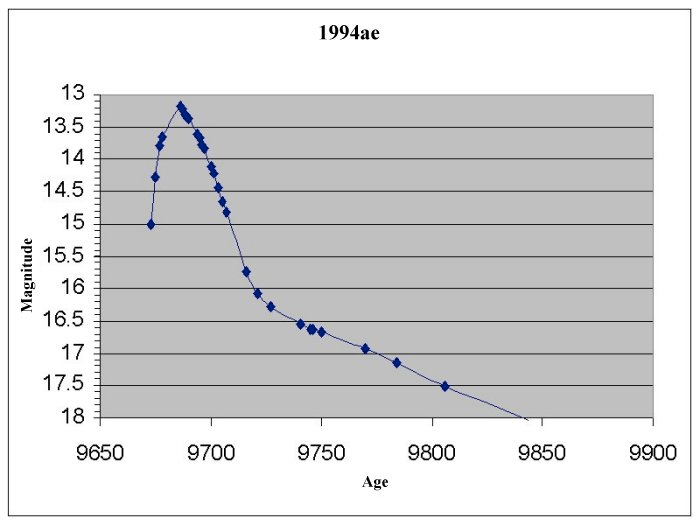
\includegraphics[width=0.7\textwidth]{dark-energy/light-curve-1994ae}
	\caption{Light curve for supernova 1994ae. The age is given in days.}\label{de:fig:light-curve}
\end{figure}

Supernova are used to measure distance in a manner similar to how we
measured distance in the Hubble lab. In the Hubble lab, we used the fact
that objects that are father away look smaller, that is, they subtend a
smaller angle on the sky. So, if we know the physical size of the object,
we can measure the object’s angular size and from that determine its
distance. For supernova, astronomers utilize the fact that objects that
are closer, look brighter, and objects that are farther away, look dimmer.
So, if we know the intrinsic brightness of an object (called its absolute
luminosity), we can then compare that to our measured brightness
(called its apparent brightness) to determine the object’s distance. This
concept for measuring distance is illustrated in Figure~\ref{de:fig:candles} showing how an object of a known brightness (or size) looks fainter
(smaller) when it is farther away.

\begin{figure}
	\centering
	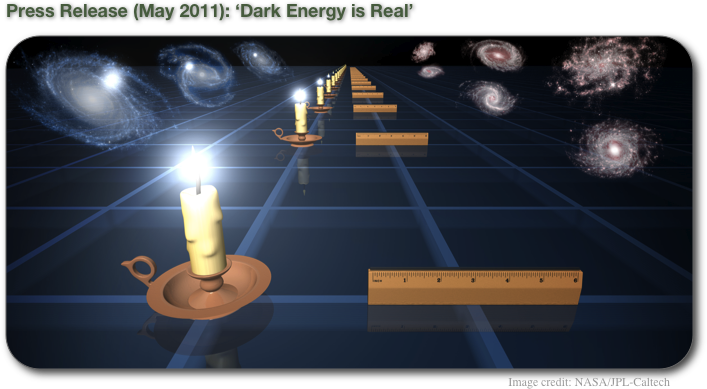
\includegraphics[width=0.8\textwidth]{dark-energy/candles}
	\caption{A method to determine the distance of an object. For objects with the same absolute luminosity, those are are further away will appear dimmer.}\label{de:fig:candles}
\end{figure}

The 1998 supernova teams studied Type Ia supernova because it is
possible to use the shape of the supernova light curve to deduce the
intrinsic brightness of the supernova. By comparing our inferred
intrinsic brightness with our measured apparent brightness, we can
then use the supernova to measure the distance.

\section{Making a supernova Hubble diagram}

The first activity for this lab is to make a Hubble diagram, like in the
Hubble lab, using Type Ia supernovae. Then you will analyze your Hubble diagram to qualitatively measure cosmic acceleration. Your data is in the Excel spreadsheet (available on Canvas in the Lab module in the compressed file DarkEnergyLab.zip) named SNe\_Reiss\_2004, and consists of distance moduli
and redshifts for 186 supernova from Reiss, et al., 2004.

As discussed above, the apparent magnitude of the supernova can be
used as a measurement of distance if we know the intrinsic brightness
(also called absolute brightness) of the supernova. In astronomy, we call
the difference between apparent and absolute brightness the “distance
modulus,” $\mu$, which is defined as
\begin{equation}
\mu = m - M \,,
\end{equation}
where $m$ is the apparent brightness (in
magnitudes), and $M$ is the absolute brightness (in magnitudes). The
distance to the object is related to the distance modulus by
\begin{equation}
 \textrm{distance} = 10^{(\mu-25)/5}\:\textrm{Mpc} \,.
\end{equation}

\begin{steps}
	\item In the spreadsheet, in a new column, calculate the distance for each supernova from the supernova’s
	distance modulus.
\end{steps}

After determining distances for objects, the next part of the Hubble
diagram involves making a measurement of the expansion of space. As
with the Hubble lab, we will estimate the expansion using the redshift
distortion of an object's spectrum. Recall that we measured the redshift
by looking for a specific spectral feature (either a dip or a peak) which
occurs at a known wavelength. A larger redshift indicates a faster recession velocity.

A constant expansion rate for the universe means that the amount of
expansion is proportional to the amount of time. Mathematically, we can
write this as
\begin{equation}
 \textrm{expansion } \propto \textrm{ time} \,.
\end{equation}
As expected, light emitted by more distant (and therefore older) objects
will undergo more expansion. This expansion leads to the redshifting
we discussed above. So, we can write that for a constant expansion rate,
the relationship between redshift and distance is
\begin{equation}\label{de:eq:hubble}
 \textrm{redshift} = \frac{H}{c} \times \textrm{distance} \,,
\end{equation}
where $c$ is the speed of light (300,000 km/s) and $H$ is called the Hubble
constant. This relation is known as “Hubble’s Law.” It describes a linear
relationship between redshift and distance, the two axes of the Hubble
diagram.

We can measure the expansion rate of the universe by using our Hubble
diagrams and fitting the data to Hubble’s law. The slope of the line that
fits the data will give a measurement of the Hubble constant, H, which
parameterizes the expansion rate of the universe.

\begin{steps}
	\item In the spreadsheet, sort data from closest to furthest. Then separately fit linear relationships to the 40 nearest and 40 furthest supernovae to obtain two Hubble constant measurements (Note that in Equation~\ref{de:eq:hubble}, the $y$-intercept is set to zero, so be sure to do this in your fit as well). Plot both linear relationships, as well as the data being fit, on a single graph. In order to see both sets of data more easily, set both axes to log scale to make a log-log plot.
	
	\item What value of the Hubble constant best fits the data for the 40
	closest supernova?
	
	\item What value of the Hubble constant best fits the data for the 40
	farthest supernova?
	
	\item How do these two results show that the expansion rate is accelerating?
	
	\item If the expansion rate is accelerating, what do you predict you
	should see if you fit data for 40 supernovae at intermediate
	distances?
	
	\item What value of the Hubble constant best fits the data for 40
	intermediate distance supernovae? Add this to your plot.
\end{steps}

\section{Finding and measuring supernovae}

Supernova are random events. In order to use supernova for
cosmological studies, astronomers must find them first. In this final
section of the lab, you will look at real data from the Dark Energy
Survey. You will search for a supernova and measure its light curve. Dr.
Daniel Scolnic, a former KICP fellow at the University of Chicago, has graciously
provided the images for this section.

\begin{steps}
	\item In the file you downloaded earlier, find the folder “SNe\_search” and
open the two image files SNe1\_search.jpeg and SNe2\_search.jpeg.
Compare these two images. These images correspond to pictures taken
of the same patch of sky on two different nights. A supernova is in one of
the images. Can you see it?
\end{steps}

In general, it is difficult to find supernova in a raw image of the sky
because of all the other objects in the image. Take a moment to look at
the different objects. Almost all of them correspond to stars
and galaxies.

Since the majority of objects in an image of the sky are not supernovae,
astronomers can try to remove them by generating a template image for
that patch of sky and then subtracting it from the image. Once these
non-supernova objects are removed (or mostly removed), it becomes
easier to search for supernovae.

\begin{steps}
	\item Open the file SNe1\_template.jpeg and compare it to SNe1\_search.jpeg.
\end{steps}
SNe1\_template.jpeg is the template file and it should look very similar
(though not exactly the same) to SNe1\_search.jpeg. Subtracting the two
yields a “difference” image which is file SNe1\_diff.jpeg.
\begin{steps}
	\item Open SNe1\_diff.jpeg.
\end{steps}
You should notice two things, 1) most of the features are now gone, and 2) the subtraction is imperfect. The imperfect subtraction introduces some artifacts in the differenced
image such as the spiderweb-like patterns and perfect geometric shapes
(like uniformly dark or bright squares and circles). You will note that
most of the artifacts from the imperfect subtraction are in locations
where there were very bright objects in the original image.

A supernova in the difference images will look like a round solid blob
that is very bright. Because a supernova is transient, the brightness of
the blob will not be the same in all images. In fact, there should be a few
images where there is no blob at all.

\begin{steps}
	\item Open the two difference images SNe1\_diff.jpeg and SNe2\_diff.jpeg.
	Compare these two difference images and identify the supernova.
	Remember, the supernova will look like a bright solid round blob in one
	of the images.
\end{steps}

Once you have found the supernova, the next step is to measure the
supernova light curve. We will do this using the DS9 software on your
computer.
\begin{steps}
	\item Open DS9 and press the “File” button to bring up the file
	menu. Press “open” and open the file 1-25-2014.diff.fits. This is the
	original file for the image with the supernova above.
\end{steps}

In DS9, you will need to press the “scale” button followed by the “zscale”
button so that the image will appear properly. You can drag the box to
look more closely at different parts of the image.
\begin{steps}
	\item Play around with the
	settings associated with the zoom, scale, and color buttons and examine
	different parts of the image.
	
	\item Find the supernova in this file (it is in the same location as in the earlier
	jpeg images). As you move the mouse around on top of the supernova,
	the “value” field will show you the value of the pixel underneath the
	mouse. Find the location on the supernova where this value is maximaland record the (X,Y) coordinates (the numbers for Image X and Y)
	below. We will use these (X, Y) coordinates as the coordinates for the
	supernova. Also record the pixel value.
	
	\item To measure the supernova’s light curve, load up each of the other *.fits
	files. Move the mouse to the (X, Y) coordinates you determined for the
	supernova and record the date and pixel value in your spreadsheet. Remember, the
	supernova is a transient object and it may not be present in all images.
	The filename tells you the date the image was taken.
	
	\item In the spreadsheet software, make a plot of the pixel value versus time. Make sure you use
	the date of the image to put your data in chronological order and to
	determine the time between each of the images.
\end{steps}

\section{Report checklist and grading}

Each item below is worth 10 points, and there is an additional 10 points for attendance and participation.

\begin{enumerate}
	\item Your Hubble diagram with all three sets of 40 supernovae and the three best-fit lines with their equations.
	
	\item Your three determinations of the Hubble constant (near, far, and mid), with work showing how you found them.
	
	\item Answers to questions 5 and 6.
	
	\item The table and plot of your experimental supernova light curve.
	
	\item Write
	one paragraph summarizing this lab. What is the significance and
	historical context of the discovery of cosmic acceleration (also called
	Dark Energy)? Why was it important? How does your analysis of the
	data in this lab demonstrate that the expansion rate of the universe is
	accelerating?
	
	\item A 100--200 word reflection on group dynamics and feedback on the lab manual. Address the following topics: who did what in the lab, how did you work together, what successes and challenges in group functioning did you have, and what would you keep and change about the lab write-up?
\end{enumerate}

%\chapter{Measuring the Cosmic Microwave Background}

%todo include continuous reading of angle and power data, maybe using video?

%todo build up to this lab using blackbody lab with light bulbs? Maybe this device and different temperatures of light bulbs and spectrometers?

\section*{Introduction}

In this experiment we will perform a measurement first carried out in the mid 1960s by Arno Penzias and Robert Wilson, for which they shared the 1978 Physics Nobel Prize for the discovery of the Cosmic Microwave Background Radiation.\footnote{A note on the Penzias and Wilson Nobel-prize winning measurement can be found at: \url{http://www.bell-labs.com/project/feature/archives/cosmology/}.}  We will measure the temperature of the Cosmic Microwave Background Radiation by comparing the  power of this emission directly with the emission from thermal sources in the lab. 

\begin{figure}[htbp]
	\begin{center}
		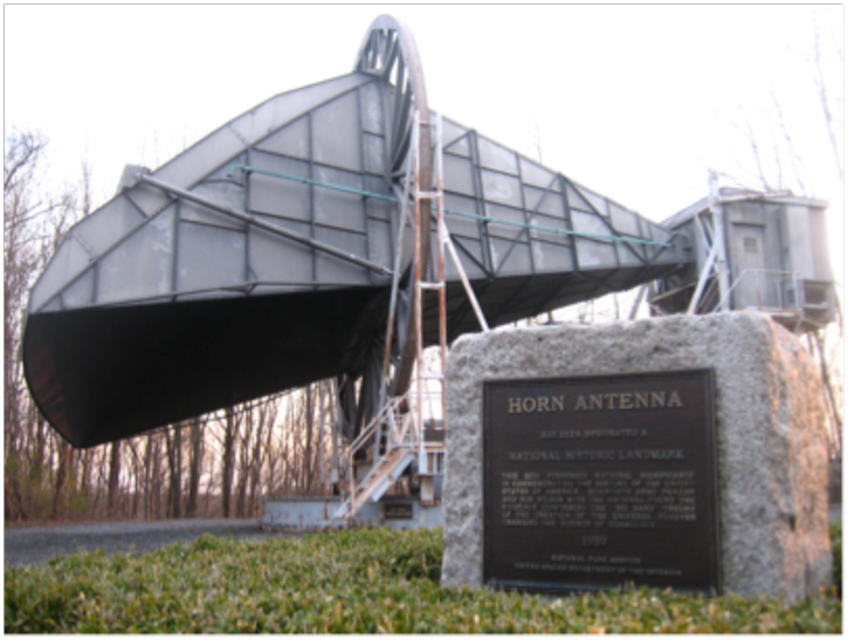
\includegraphics[width=.45\textwidth]{cmb/CMB-horn-antenna.pdf}
		\caption{A photo of the horn antenna with which Arno Penzias and Robert Wilson discovered the Cosmic Microwave Background radiation. This lab uses a smaller horn working at a much higher frequency (shorter wavelength), so that the ``beam patterns" are similar (recall the Small Radio Telescope lab and beam measurements to see why). }
		\label{fig:PW-horn}
	\end{center}
\end{figure}

\section{Measuring Temperatures with Thermal Radiation}

We use the basic fact that at sufficiently long wavelengths, the power emitted by a perfect thermal emitter is proportional to the temperature of the emitter:
\begin{equation}
P = \alpha T
\label{one}
\end{equation}
where $P$ is the power emitted, $\alpha$ is a constant that depends on area, wavelength, and other factors, and $T$ is the physical temperature of the emitter in Kelvin. 

To measure the power we use an instrument that can measure the incoming radiation power and it has input optics arranged so that it ``views'' a small range of angles in front of the instrument. This is the basis of a radiometer. You can imagine this as a reverse flashlight. In the case of the flashlight, the filament of the light bulb is hot and emits through an arrangement of mirrors to form a narrow beam. For the radiometer, the ``heat radiation'' from a narrow range of angles funnels into the instrument and the power is detected and the amount of power read out on a meter.

In practice, the receiver used to measure radiation is not perfect and generates some `noise' power of its own. So even if we pointed the receiver at an object with $T=0$, it would still measure some power. This extra power is denoted in terms of the temperature, $T_\textrm{rx}$, you would measure if you looked at a zero temperature emitter and did not correct for this fact:
\begin{equation}
P = \alpha (T + T_\textrm{rx}).
\label{two}
\end{equation}

To compute temperature of an emitter, $T$, from the power, $P$, measured by receiver, we need to know $\alpha$ and $T_\textrm{rx}$. 
It would be hard to calculate the factor $\alpha$ from first principles, especially because in order to be useful the calculation must include all of the details of the measuring equipment.  However, it is straightforward to obtain an accurate measurement of  $\alpha$ experimentally by measuring the power for different temperatures.

We will determine the factor $\alpha$ by placing first an emitter of one known temperature in front of the radiometer, noting the power reading on the meter, then placing a different emitter with a different known temperature in front of the radiometer and noting the new power level. According to equations~\ref{one} and \ref{two}, these two measurements can be used to calculate $\alpha$:
\begin{equation}
\alpha = {P_1 - P_2 \over T_1 - T_2}
\label{three}
\end{equation}

Once $\alpha$ is calculated, we can solve for $T_\textrm{rx}$ from measurement of one of the known temperature emitters:
\begin{equation}
T_\textrm{rx} = {P_1 \over \alpha} -T_1
\label{four}
\end{equation}
With $\alpha$ and $T_\textrm{rx}$ measured, we can ``point'' the radiometer anywhere and remotely measure the temperature of any emitter corresponding to the received power $P$ by solving eq.~\ref{two}  for $T$,

\begin{equation}
T={P\over \alpha} - T_\textrm{rx}
\label{five}
\end{equation}

Note that when you will be measuring the temperature of the ``hot'' load you will need to convert the temperature in degrees Celsius or Fahrenheit it reports into Kelvins.

\section{The receiver and experimental set up}

Figure~\ref{fig:CMBLab-photo} shows the experimental set up you will be using in this lab. The 30 GHz receiver is enclosed in a cryostat enclosure that keeps it very cold to reduce its noise. It is mounted on a cart in a contraption that allows to change its pointing for different elevations. Radiation measured by the receiver enters through receiver window at the top of the enclosure. The power measured by the receiver is displayed in digital form on the power readout screen. Pointing of the receiver can be changed using the elevation control lever and current elevation can be read on the electronic angle meter mounted on the enclose (this meter should be calibrated at the zero angle at the beginning of the lab with the help of your TA).

Figure~\ref{fig:schematic} shows details of the receiver when it is taken out of the cryostat enclosure.

\begin{figure}[ht]
	\begin{center}
		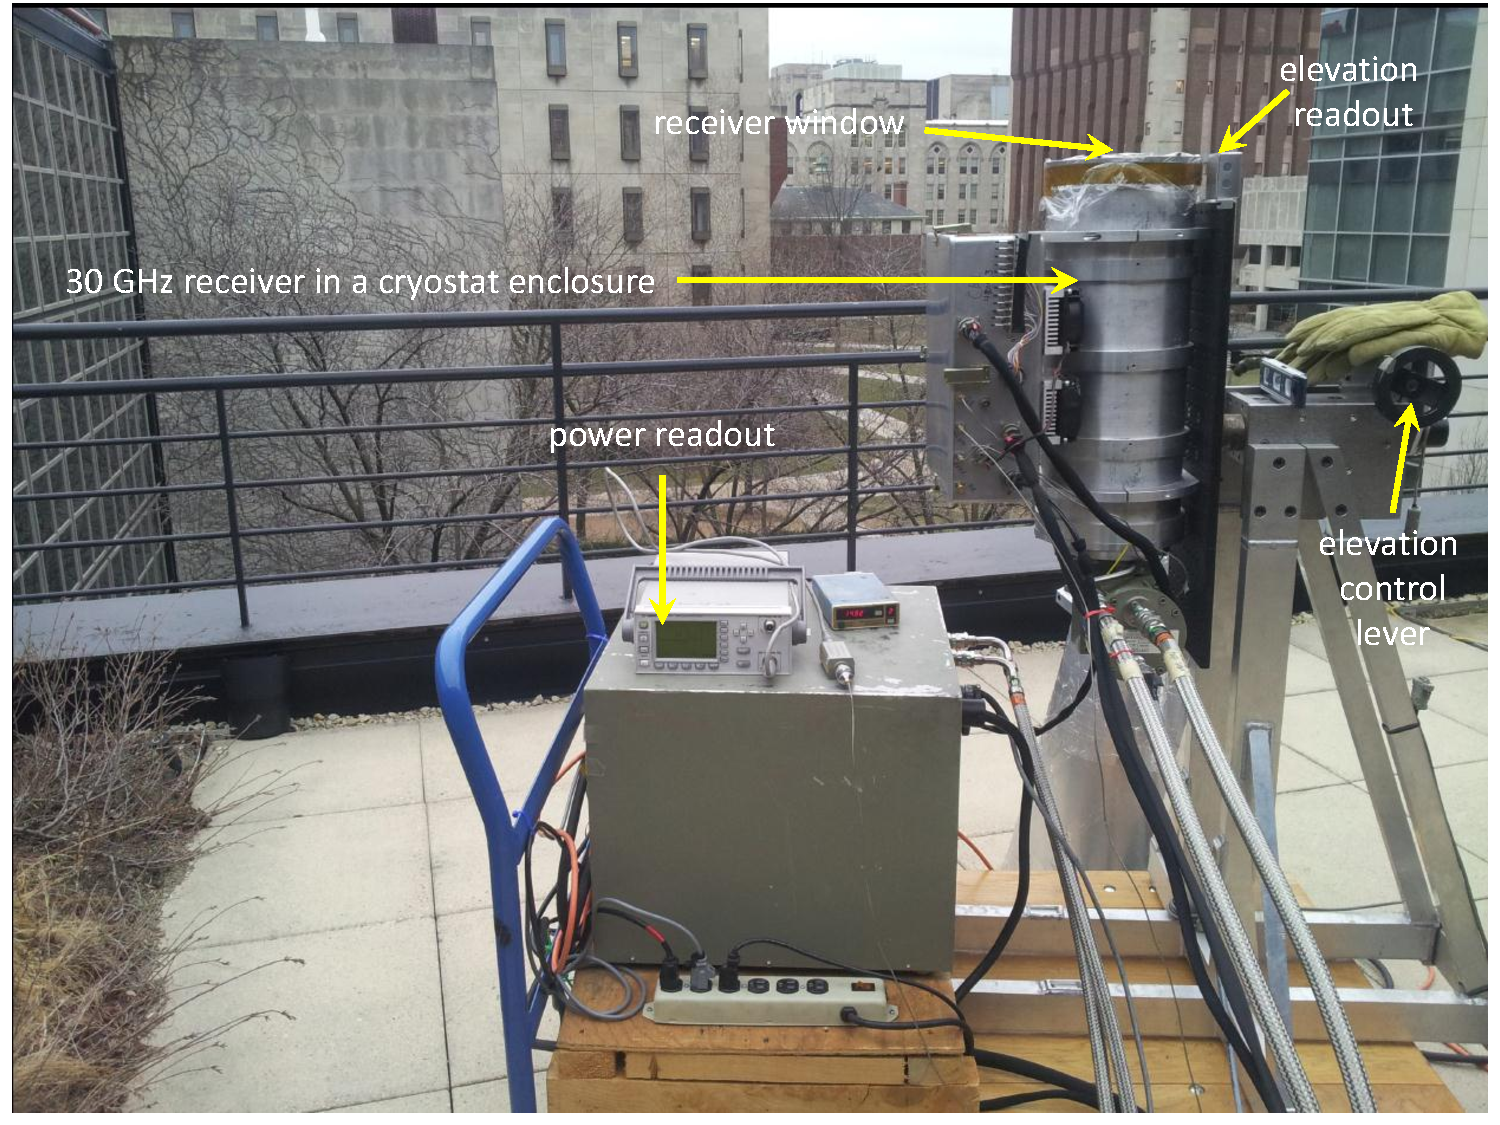
\includegraphics[trim=0pt 0pt 0pt 0pt,width=0.9\textwidth]{cmb/receiver_setup_new.pdf}
		\caption{Photo of the 30 GHz receiver enclosed in a cryostat enclosure mounted on the cart. This set up on a patio of KPTC 312 will be used in this lab for measurements of temperature of the sky.}
		\label{fig:CMBLab-photo}
	\end{center}
\end{figure}

\begin{figure}[htb]
	\begin{center}
		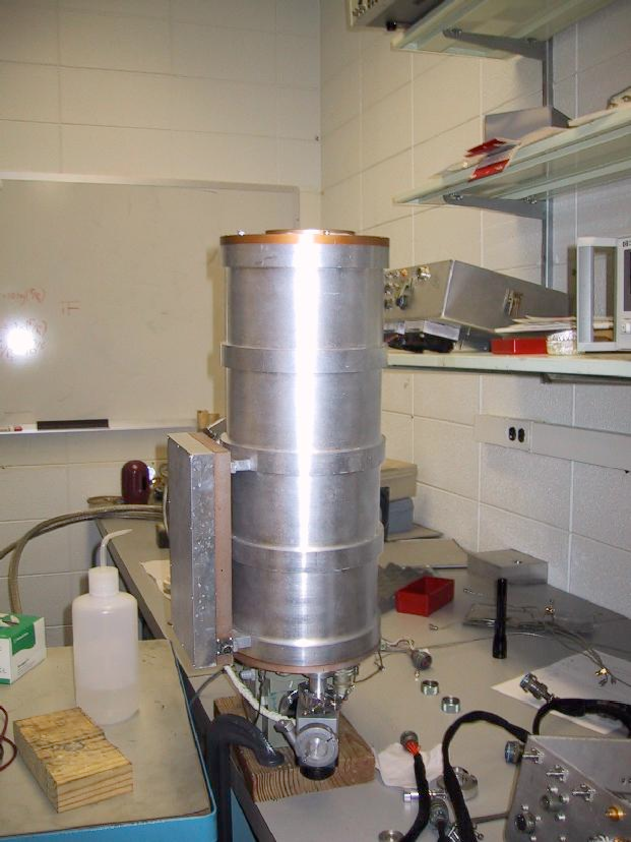
\includegraphics[trim=0pt 0pt 0pt 0pt,width=0.4\textwidth]{cmb/SZ-Cryostat-Closed.pdf}
		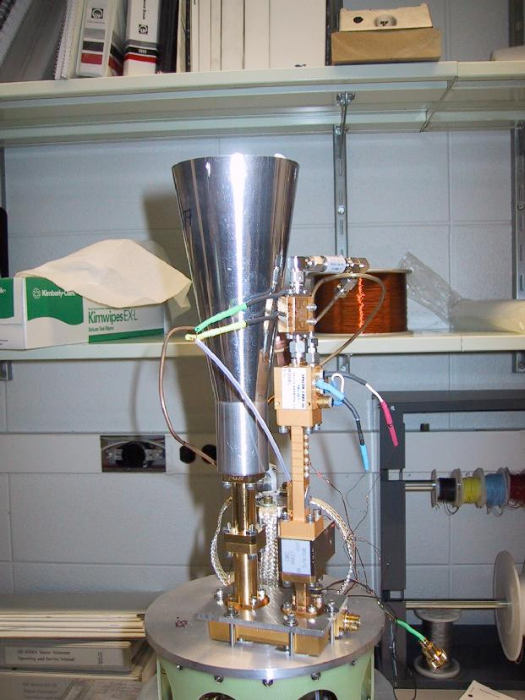
\includegraphics[trim=0pt 0pt 0pt 0pt,width=0.4\textwidth]{cmb/SZ-Cryostat-Open.pdf}
		\caption{\textit{Left:} The CMB lab 30 GHz receiver closed in the lab. \textit{Right:} A photo of the inside of the cryostat showing the  horn and electronics of the receiver.  The outer shell of the cryostat provides the vacuum seal for the interior components that are cooled to roughly 15 K (-258 C) inside of thermal radiation shields (not shown) to lower the noise generated by the electronics, and even the noise due to the radiation from the horn. The electronics amplify the signal by roughly a factor of 10,000.  By cooling and using a specially designed amplifier for this research, the receiver only adds a small amount of noise, roughly equivalent to that which would result by placing 10 K at the input of an idealized noiseless receiver (if only such things existed!). This receiver  was built here at the university and is also used to at the CARMA radio astronomy observatory, see \url{http://www.mmarray.org/}, for which The University of Chicago is a partner. It is one of a handful of the most sensitive 30 GHz receivers in the world.}
		\label{fig:schematic}
	\end{center}
\end{figure}

\section{Measuring the Temperature of Items in the Lab}

We will first measure the temperature of several items using the radiometer. 

Some things you could measure: 
\begin{enumerate}
	\item The wall or ceiling
	\item The sky through the door of the lab
	\item Your cupped hands above the receiver or your face
\end{enumerate}

For each item, you should make three or more measurements quickly in succession of the cold load, the hot load, and the source for which you want to measure temperature. The hot load is a piece of material that is a good emitter and the temperature is near room temperature and is measured with a a digital thermometer located at the top of the load (see left panel of Fig.~\ref{fig:details}). The cold load is a similar material that is first immersed completely in liquid Nitrogen (which has temperature $T_\textrm{cold}=77.4$~K),\footnote{It is important that the entire cone is immersed in the liquid Nitrogen or else the effective temperature of the load will be poorly determined and this will lead to incorrect measurement of the source temperature.} as shown in the middle panel of Fig.~\ref{fig:details}. When you are ready to make a measurement with the cold load, take it out of the dewar, let the liquid Nitrogen drip for $\sim$5 seconds and place it in front of the receiver window. Be careful to fully cover the window, but do not rest the cold load on the cryostat. Then comes the source of unknown temperature. For each of these objects you will need to read the power reading on the power meter attached to the receiver (see Fig.~1).

Find the unknown temperature using equation~\ref{two} to find $\alpha$, equation~\ref{four} to find $T_\textrm{rx}$, with $T_1$ and $P_1$ being the temperature and power for the hot load, $T_2$ and $P_2$ being the temperature and power for the cold load. Then using equation~\ref{five}, find the unknown temperature using the power measured while the unknown was in front of the receiver.

\begin{figure}[ht!]
	\begin{center}
		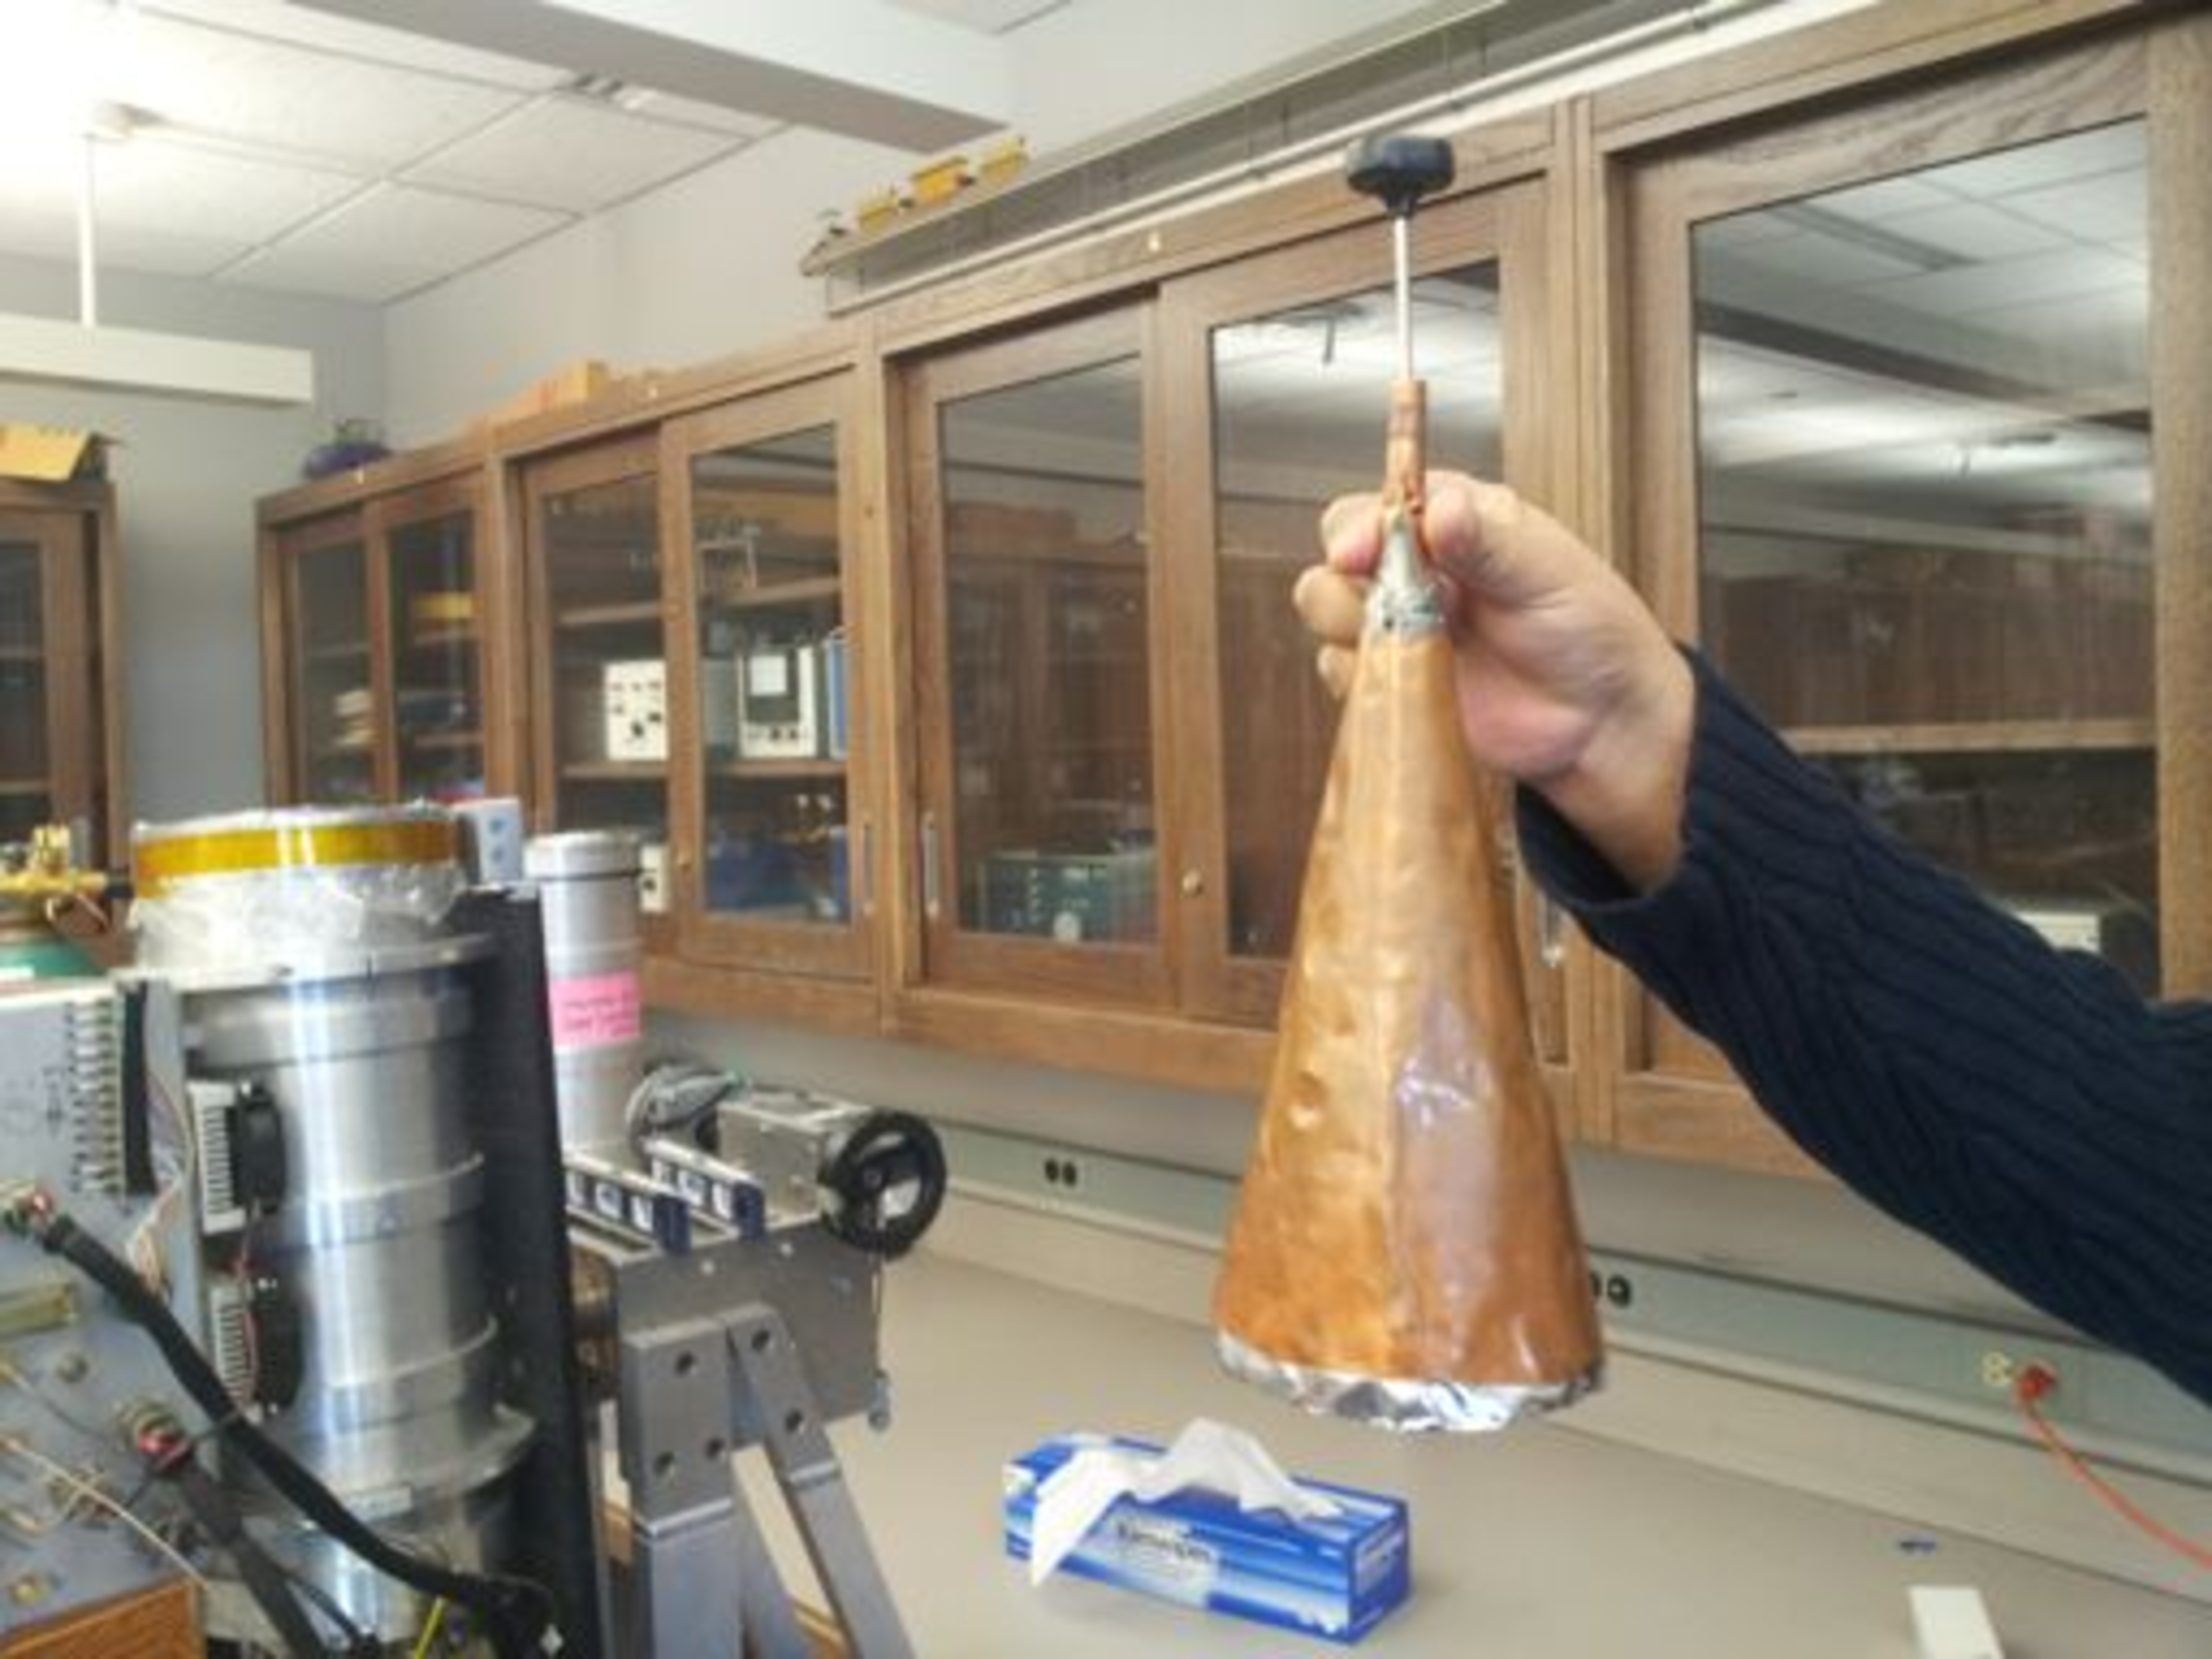
\includegraphics[trim=0pt 0pt 0pt 0pt,width=0.32\textwidth]{cmb/hot_load-small.pdf}
		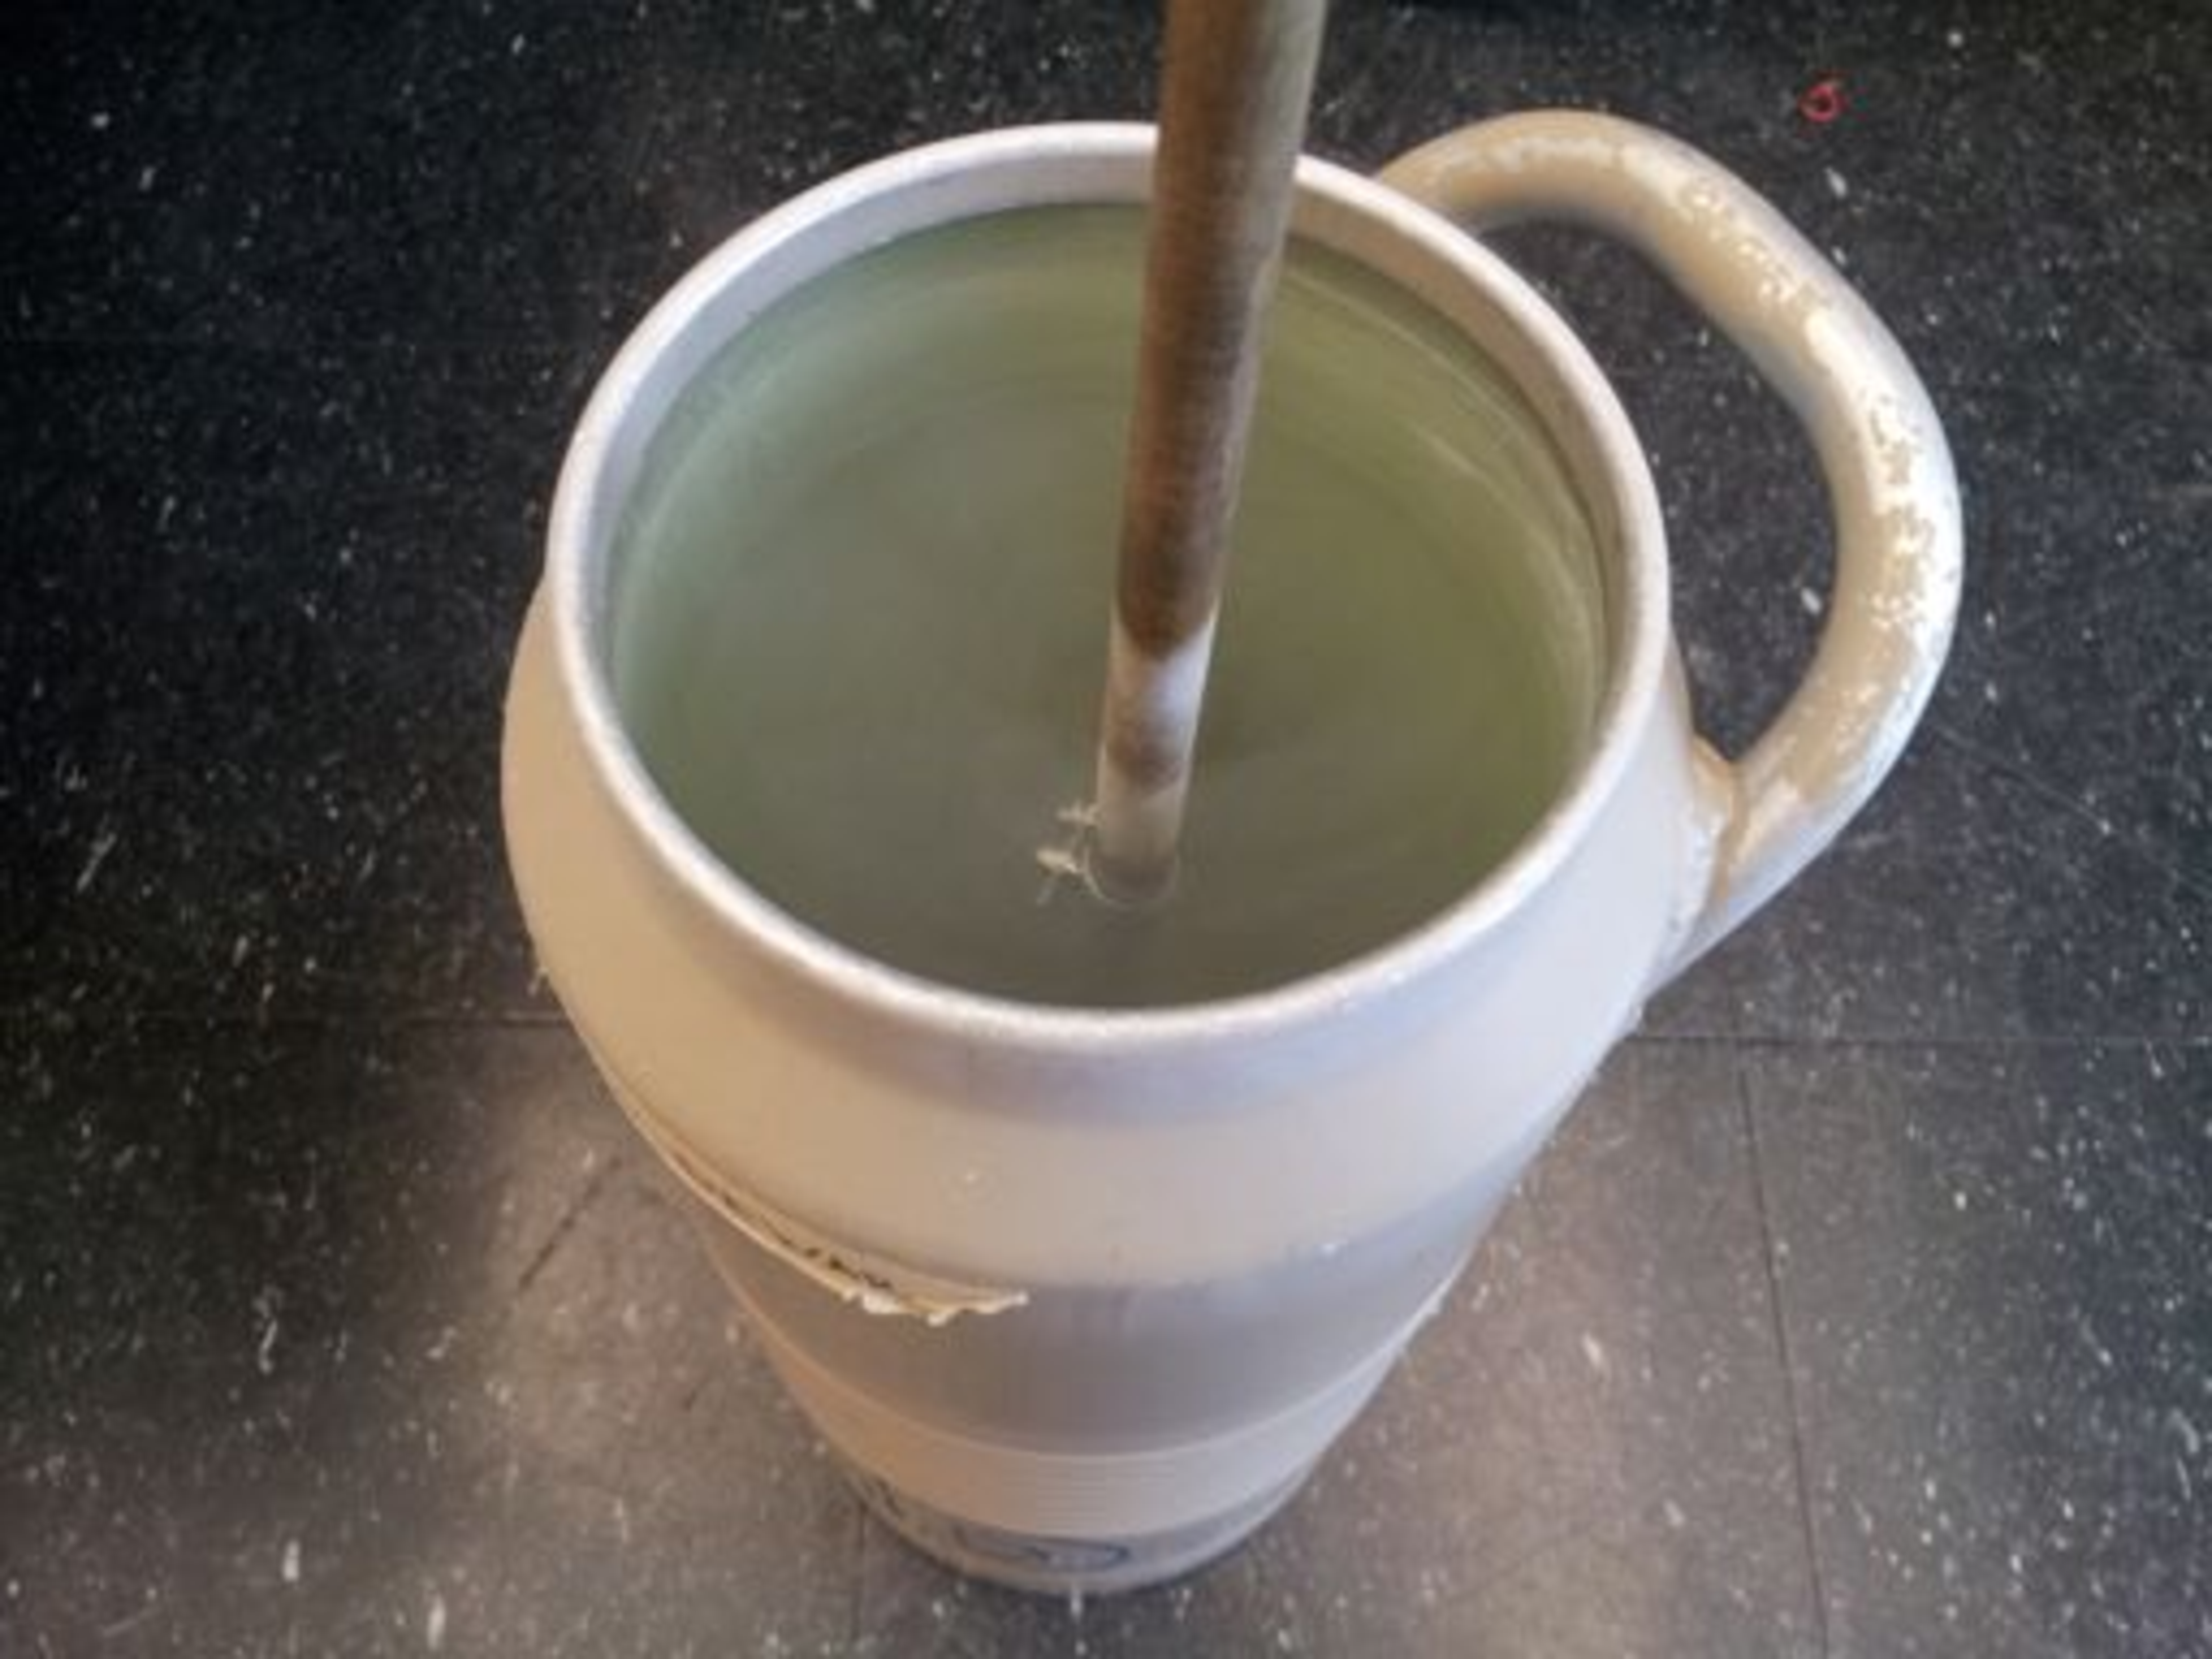
\includegraphics[trim=0pt 0pt 0pt 0pt,width=0.32\textwidth]{cmb/cold_load-small.pdf}
		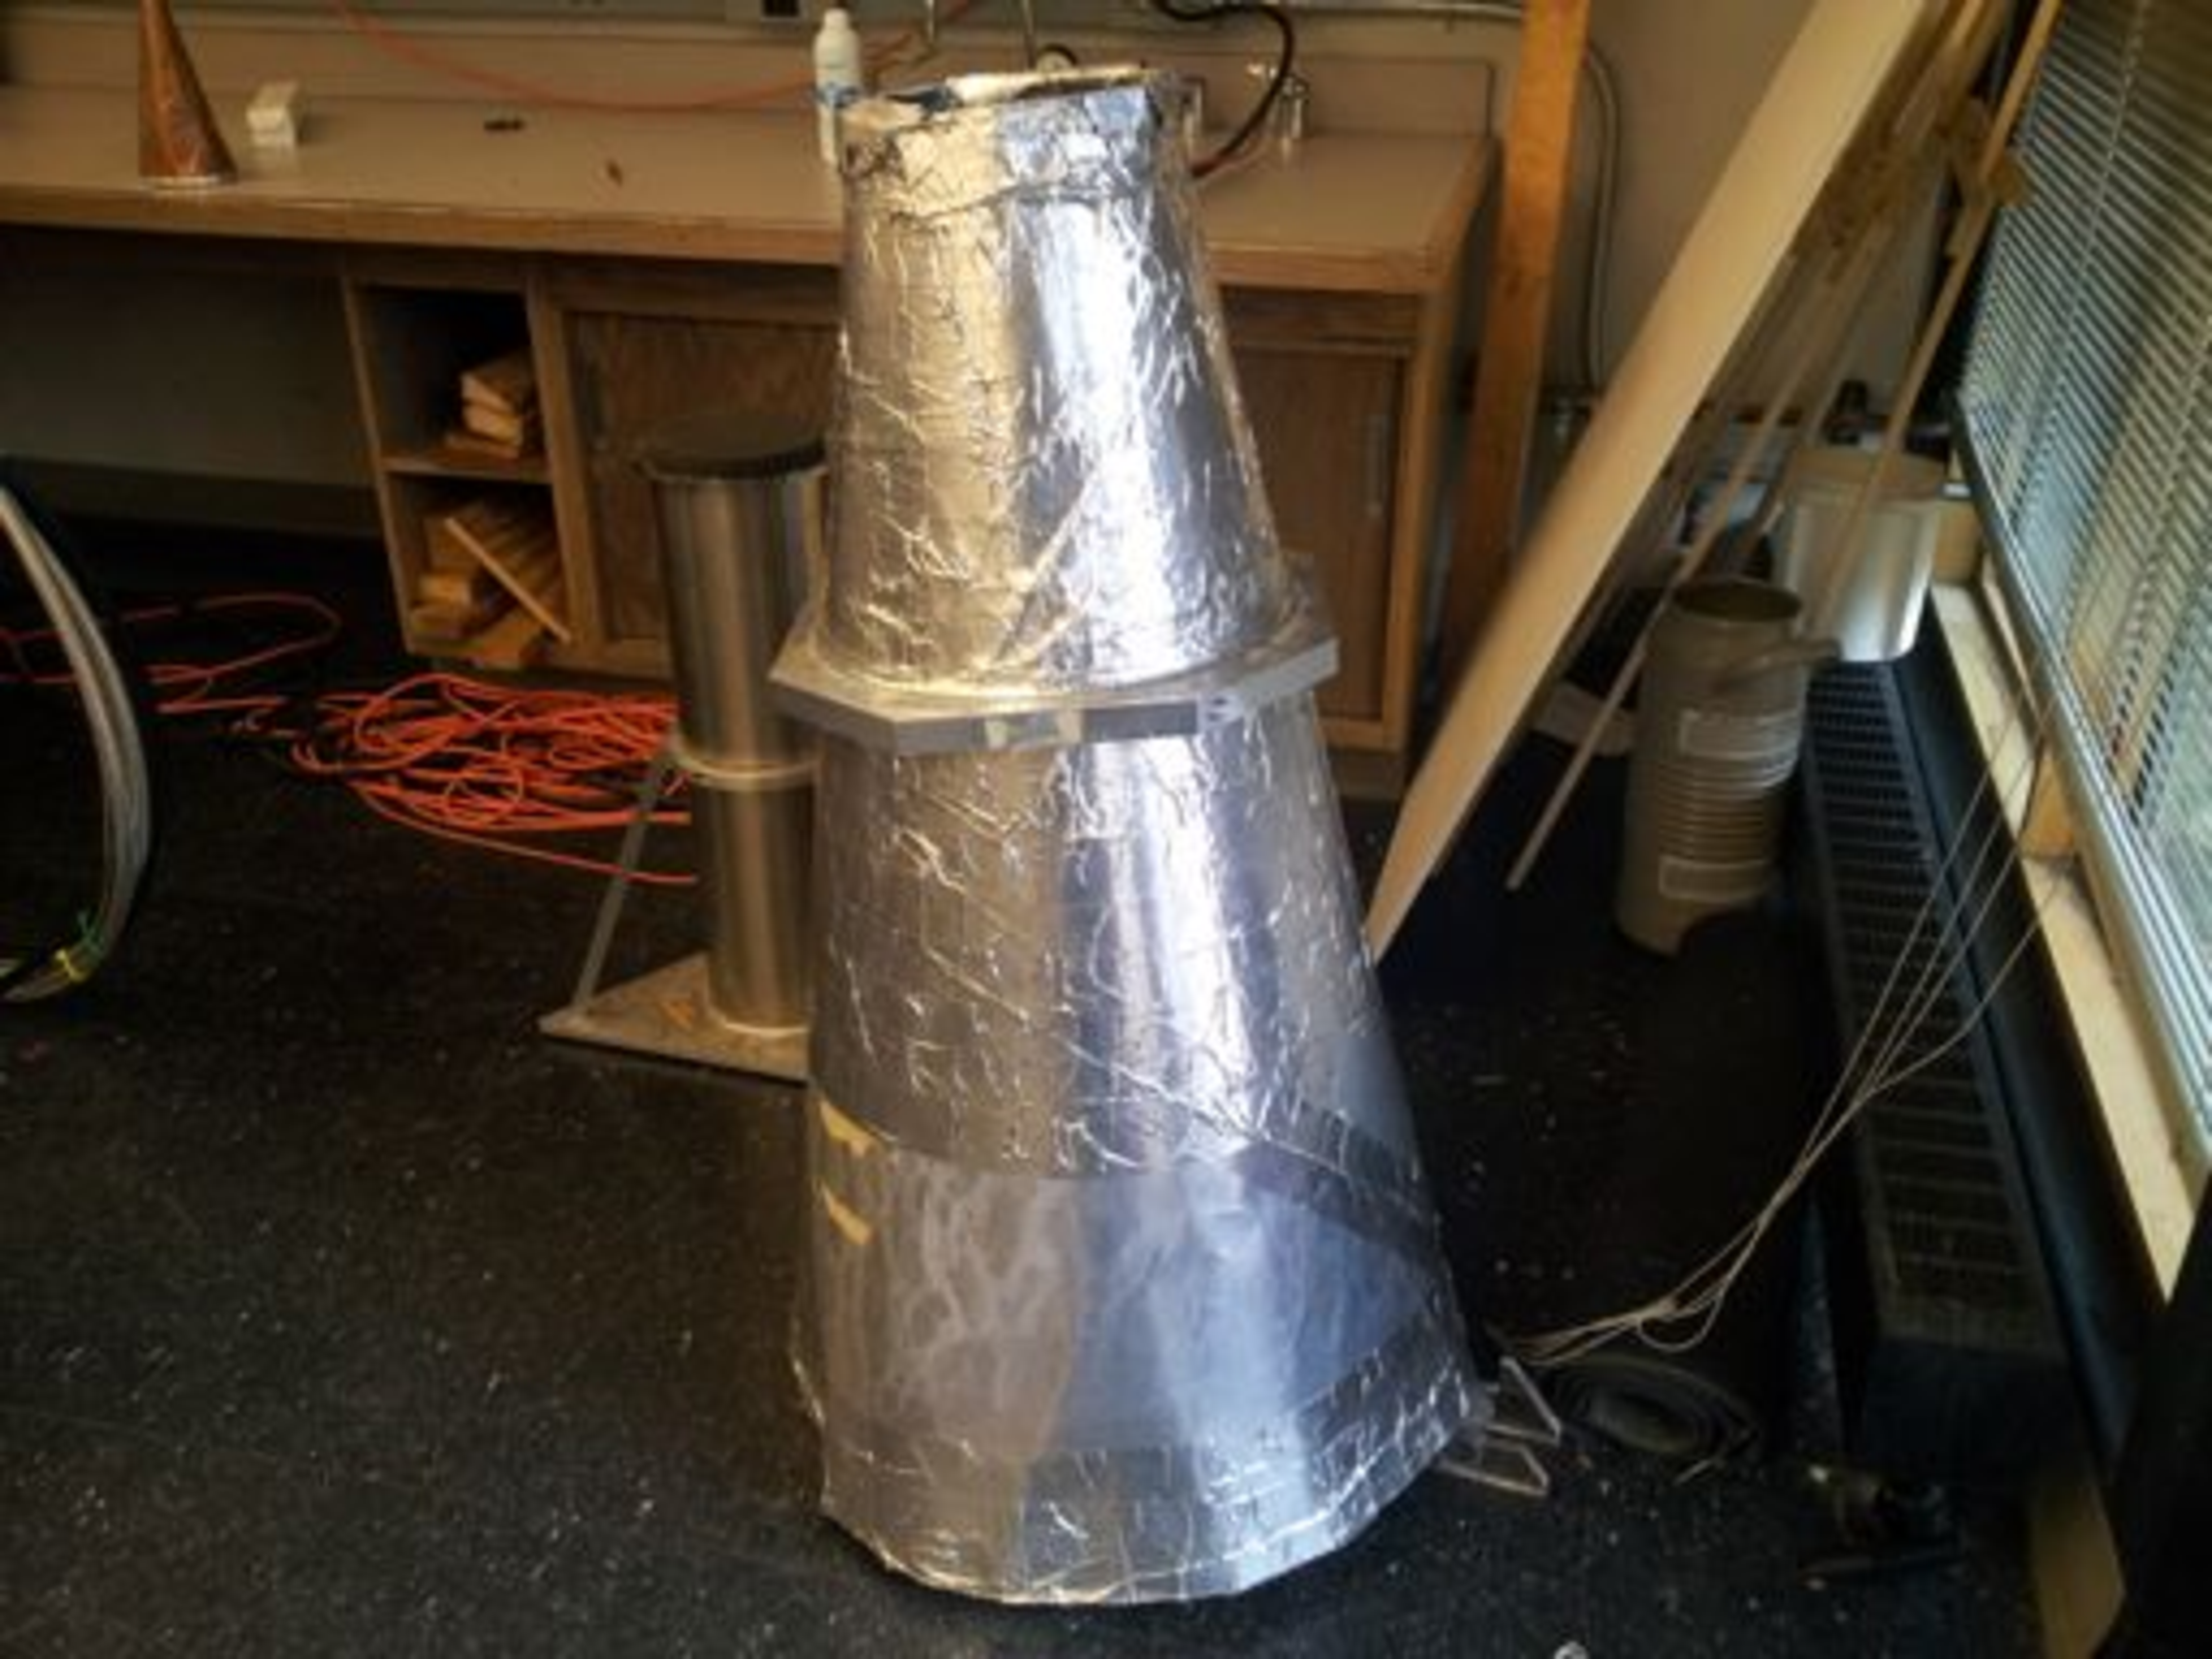
\includegraphics[trim=0pt 0pt 0pt 0pt,width=0.32\textwidth]{cmb/ground_shield-small.pdf}
		\caption{\textit{Left:} The ``hot'' load with digital thermometer at the top. \textit{Center:} ``cold'' load submerged in a dewar with liquid Nitrogen. Make sure that the cooper part of the load is fully submerged with the liquid surface at a wooden part of the load. \textit{Right:} ground shield which will be used to minimize radiation from nearby buildings  and the ground when measuring radiation from the sky. } 
		\label{fig:details}
	\end{center}
\end{figure}

\section{Measuring the Temperature of the CMB}

Measuring the temperature of the CMB is conceptually the same as  measuring the temperature of the items in the lab. We will compare the power we get from the sky to the hot and cold loads.

Because the CMB temperature is very low (just a few degrees K) we have to take a more careful account of a few things than we did for the previous section. First, we will have to get $T_\textrm{rx}$ pretty accurately because the CMB temperature, $T_\textrm{CMB}$ is less than $T_\textrm{rx}$. Second, there are hot sources (compared to the CMB) all around the experiment. You can imagine that even a small bit of one of these hot sources in part of the beam would change the oncoming power a lot and cause a big change in what we infer for the CMB temperature. 

We will also have to worry about two other sources.
One is the hot ground and buildings around us. We will guess about these sources by placing a ground shield on the receiver, which keeps the ground emission out of the input (see right panel of Fig.~\ref{fig:details} to see how the ground shield looks like). We will check how much difference this makes and subtract that source if it seems to be an important factor.

The second, and more difficult extraneous source to remove is emission from our own atmosphere. While the atmosphere is \textit{almost} transparent (and therefore almost non-emissive), it is not perfect. What's more, the main emitter is water-vapor which varies a lot. There is not much water vapor on those clear, crisp days when the sky is deep blue. On the other hand, when it's wet and cloudy, there is a lot of water vapor, and consequently, if we point our radiometer up at the sky we will get a hotter temperature on humid or wet days.  

As you also know water vapor is not well mixed in our atmosphere (e.g. clouds), so on a poor day you will see the output power of the radiometer changing quickly as the winds blows different blobs of water vapor in front of the radiometer.  Try comparing the stability of the radiometer when staring at the warm load compared to staring at the sky. On a good day the power when staring at the sky is as stable as that when staring at the load.

How can we estimate the amount of power coming from the atmosphere when we point the radiometer at the sky? We need to do this to get a good estimate of $T_\textrm{CMB}$. We do this by measuring the effective temperature as a variety of angles from the vertical. We can calculate how much atmosphere we are going through for each angle and from that, extrapolate the temperature we would get if were looking through zero atmosphere. The atmosphere contribution approximately follows
\begin{equation}
T_\textrm{atm}(z) = T_0 A(z)
\end{equation}
where $A(z)$ is the number of airmasses you are looking through. $A(z)=\sec(z)$, where $\sec(z)=1/\cos(z)$ is the secant function -- reciprocal of the cosine function and is equal to 1 when looking straight up ($z=0$).
$T_0$ is the atmosphere temperature at the zenith and $z$ is zenith angle (the angle between straight up and where the radiometer is looking). The total temperature we will measure when looking at the sky (after subtracting $T_\textrm{rx}$ according to equation~\ref{five}) will be 
\begin{equation}
%T_{\rm total} = T_{\rm CMB} + T_{\rm atm}(z) + T_{\rm rx}
T_\textrm{total} = T_\textrm{CMB} + T_\textrm{atm}(z)
\label{seven}
\end{equation}

\begin{framed}
To get an estimate of $T_\textrm{CMB}$, we will measure the $T_\textrm{total}$ at a variety of zenith angles. We then plot $T_\textrm{total}$ vs $A(z)$ to get a straight line for $A(z)$ going from 1 to about 2 ($z$ going from 0 to 60$^\circ$). Then we can extrapolate the straight line to $A=0$ and read off $T_\textrm{CMB}$.
\end{framed}

A flow chart of the measurement strategy is shown in Figure~\ref{fig:flow-chart}. It is important to understand the quality of the data as you take it -- your TA will help you with this. There are many reasons the data could be corrupted, e.g., poor cold load temperature if not well immersed in liquid Nitrogen, the radiometer not being leveled, not centering the loads on the window or aligning the reflecting shield along the beam, buildings in the way, poor  and unstable atmospheric transmission, etc.
Good zenith angles to give well sampled air mass measurements are: $0^o,~15^o,~25^o,~35^o,~40^o,~45^o,~48^o,~52^o,~54^o,~56^o,~58^o,~60^o$, although you may find that the buildings do not allow good results at the higher zenith angles, even after correcting for the sidelobe response (see below).   Be sure to 
measure $T_{total}$ at each of the zenith angles with the hot load  -- cold load -- hot load method as shown in the flow chart.  

Because the receiver has some sensitivity to emission from angles far outside of its beam referred to as the beam sidelobe response (and at extreme angles as the far sidelobe response),  it is important to account for the excess power picked up by the sidelobe response from the warm buildings, the ground and also the Sun. We do this by making measurements at each zenith angle with the   ``ground shield" (see right panel of Fig.~\ref{fig:details}).  Once the sky and load measurements are obtained at a given zenith angle, take several measurements in quick succession of the power on the sky with the ground shield off and placed along the beam axis.  If the shield is well aligned (use two spotters to make sure it is), then the receiver output power will be lower when the shield is in place, especially at lower elevations (higher zenith angles) due to emission from the warm buildings.  Determine the percentage change to the sky power for each zenith angle. You then correct the power in Eq.~\ref{five} before calculating the $T_{total}$ for Eq.~\ref{seven}.

Note, because of the sidelobe response, it is important that everyone is far from beam of the receiver when you are taking measurements. It is best for everyone to stay behind the plane defined by the front of the receiver. 

During the measurements, different students in the lab will take on a particular role to handle hot or cold load, read off power, put on ground shield, record the data.
\begin{steps}
	\item\label{cmb:step:table} Your measurements should be recorded in a table, which has elevation, power for the cold load, power for the hot load, temperature of the hot load read off at each measurement, power of the sky without shield, power of the sky with shield. You will take the measurements jointly but will analyze them to measure $T_\textrm{CMB}$ on your own.
\end{steps}
%There are a few other corrections we could make which will be discussed in lab.

%\newpage



%\newpage
\begin{figure}
	\begin{center}
		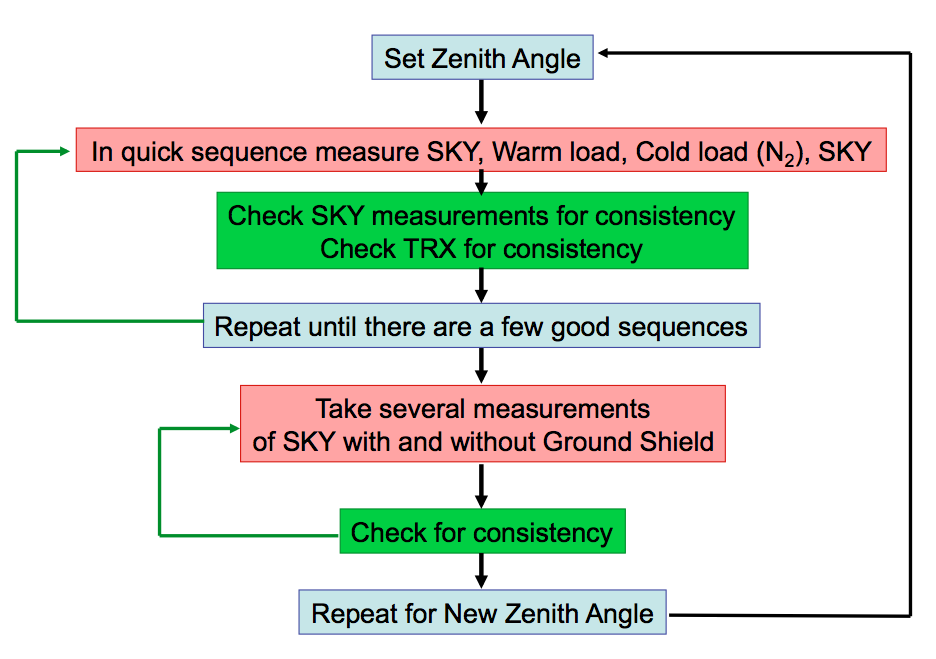
\includegraphics[trim=0pt 0pt 0pt 0pt,width=0.95\textwidth]{cmb/cmb-lab-flow-chart.png}
		\caption{Flow chart for taking sky data. It is important to make sure you obtain consistent results for each elevation angle. The ratio of the power on ambient to liquid nitrogen load should be very stable, since the scale factor $\alpha$ in Eq.~\ref{one} cancels in the ratio.  If the ratio is not stable there is a problem with the instrument (or liquid nitrogen load was not full immersed) and you will not get reliable results for Cosmic Microwave Background results.  The ratio of the output power for the ambient load to the nitrogen cooled load should be about 3.4 to 3.6, depending on the temperature of the ambient load. The typical receiver temperature should be around 11 K.  On a cloudy day the sky measurements may not be stable enough to achieve reliable results.  Why is that? \textit{Hint, light at cm wavelengths is also known as microwave radiation.  What is it that your microwave oven is heating up? And, if it absorbs the microwave radiation, then it must also emit it.}}
		\label{fig:flow-chart}
	\end{center}
\end{figure}

\section{Analysis}

\begin{steps}
	\item\label{cmb:step:plot} Plot your data, $T_\textrm{Sky}$ vs. airmass, with airmass on the horizontal axis. Airmass is defined as
	\begin{equation}
	 A(z) = \sec(z),
	\end{equation}
	where $z$ is the elevation angle.
	
	\item\label{cmb:step:fit} Fit your data to a line and record the slope and intercept for the line. \textit{Tip: double check your units. For elevation angle, we usually measure angles in degrees, but most calculators expect units of radians. Also, we will measure all temperatures in Kelvin.}
\end{steps}

\section{Report checklist and grading}

Each item below is worth 10 points, and there is an additional 10 points for attendance and participation.

\begin{itemize}
	\item Data and determination of temperature of two items inside the lab.
	
	\item Data table from Step~\ref{cmb:step:table}.
	
	\item The plot and fit parameters from Steps~\ref{cmb:step:plot} and \ref{cmb:step:fit}.
	
	\item Does your data agree with the model where the emission is dominated by the atmosphere?  What value to get for any residual temperature ($T_\textrm{CMB}$) and how do you interpret it?
	
	\item What are some of the uncertainties associated with your measurement? What steps did you take to measure or mitigate these uncertainties?
	
	\item Write a paragraph discussing the quality of your data and the historical significance of the Penzias and Wilson measurement. Include a discussion of the following: What was the context of the Penzias and Wilson measurement? Why was this measurement important? What were some of the competing cosmological theories at that time and how did the Penzias and Wilson measurement fit in to that context?
\end{itemize}

\appendix

% This format is not a formal report, but simply answering questions, including figures, and demonstrating scientific abilities.
\chapter{Lab Report Format}\label{cha:lab-report-format}

%TODO Make firm page limit? 5 pages + figures and tables?

%In a general sense, the labs should demonstrate the rubric rows listed in the lab write-up and provide answers to every lab question asked.

\section{General}

\begin{itemize}
	\item The report should be typed for ease of reading. Text should be double-spaced, and the page margins (including headers and footers) should be approximately $2.5\:$cm, for ease of marking by the grader. Each page should be numbered.
	
	\item The first page should include the title of the lab; lab section day, time, and number; and the names of the members of your lab team.
	
%	\item If the rubric row refers to a particular part of your lab report, clearly label that part of the report with that rubric row. For example, you should label the section where you demonstrate uncertainty propagation with ``G2'' if that rubric row is being assessed in that lab.
\end{itemize}

\section{Organizing the report}

%If the lab is clearly framed as an observational, testing, or application experiment, you can follow the corresponding rubric for the elements to include in the report (see, respectively, Rubrics B, C, and D in Appendix~\ref{cha:rubrics}).

The report should follow the sequence of the report checklist. Answers to questions and inclusion of tables and figures should appear in the order they are referenced in the manual. In general, include the following:

	\begin{itemize}
%		\item Any procedure that you performed that is different from what is described in the lab manual.
		
%		\item Any data that you've collected: tables, figures, measured values, sketches. Whenever possible, include an estimate of the uncertainty of measured values.
		
		\item For any calculations that you perform using your data, and the final results of your calculation, you must show your work in order to demonstrate to the grader that you have actually done it. Even if you're just plugging numbers into an equation, you should write down the equation and all the values that go into it. This includes calculating uncertainty and propagation of uncertainty.
		
		\item If you are using software to perform a calculation, you should explicitly record what you've done. For example, ``Using Excel we fit a straight line to the velocity vs. time graph. The resulting equation is $v = (0.92\:\mathrm{m/s^2}) t + 0.2\:\mathrm{m/s}$.''
		
		\item Answers to any questions that appear in the lab handout. Each answer requires providing justification for your answer.
		
%		\item At the end of each experiment, you should discuss the findings and reflect deeply on the quality and importance of the findings%
		% (Rubric Row F2)
%		. This can be both in the frame of a scientist conducting the experiment (``What did the experiment tell us about the world?'') and in the frame of a student (``What skills or mindsets did I learn?'').
	\end{itemize}

\section{Graphs, Tables, and Figures}

Any graph, table, or figure (a figure is any graphic, for example a sketch) should include a caption describing what it is about and what features are important, or any helpful orientation to it. The reader should be able to understand the basics of what a graph, table, or figure is saying and why it is important without referring to the text. For more examples, see any such element in this lab manual.

Each of these elements has some particular conventions.

\subsection{Tables}

A table is a way to represent tabular data in a quantitative, precise form. Each column in the table should have a heading that describes the quantity name and the unit abbreviation in parentheses. For example, if you are reporting distance in parsecs, then the column heading should be something like ``distance (pc)''. This way, when reporting the distance itself in the column, you do not need to list the unit with every number.

\subsection{Graphs}

A graph is a visual way of representing data. It is helpful for communicating a visual summary of the data and any patterns that are found.

The following are necessary elements of a graph of two-dimensional data (for example, distance vs. time, or current vs. voltage) presented in a scatter plot.

\begin{itemize}
	\item \textbf{Proper axes.} The conventional way of reading a graph is to see how the variable on the vertical axis changes when the variable on the horizontal axis changes. If there are independent and dependent variables, then the independent variable should be along the horizontal axis.
	
	\item \textbf{Axis labels.} The axes should each be labeled with the quantity name and the unit abbreviation in parentheses. For example, if you are plotting distance in parsecs, then the axis label should be something like ``distance (pc)''.
	
	\item \textbf{Uncertainty bars.} If any quantities have an uncertainty, then these should be represented with so-called ``error bars'', along both axes if present. If the uncertainties are smaller than the symbol used for the data points, then this should be explained in the caption.

\end{itemize}

\chapter{Analysis of Uncertainty}

A physical quantity consists of a value, unit, and uncertainty.
For example, ``$5 \pm 1\,$m'' means that the writer believes the true value of the quantity to most likely lie within 4 and 6 meters\footnote{The phrase ``most likely'' can mean different things depending on who is writing.
	If a physicist gives the value and does not given a further explanation, we can assume that they mean that the measurements are randomly distributed according to a normal distribution around the value given, with a standard deviation of the uncertainty given.
	So if one were to make the same measurement again, the author believes it has a 68\% chance of falling within the range given.
	Disciplines other than physics may intend the uncertainty to be 2 standard deviations.}.
Without knowing the uncertainty of a value, the quantity is next to useless.
For example, in our daily lives, we use an implied uncertainty.
If I say that we should meet at around 5:00 pm, and I arrive at 5:05 pm, you will probably consider that within the range that you would expect.
Perhaps your implied uncertainty is plus or minus 15 minutes.
On the other hand, if I said that we would meet at 5:07 pm, then if I arrive at 5:10 pm, you might be confused, since the implied uncertainty of that time value is more like 1 minute.

Scientists use the mathematics of probability and statistics, along with some intuition, to be precise and clear when talking about uncertainty, and it is vital to understand and report the uncertainty of quantitative results that we present.

\section{Types of measurement uncertainty}

For simplicity, we limit ourselves to the consideration of two types of uncertainty in this lab course, instrumental and random uncertainty.

\subsection{Instrumental uncertainties}

Every measuring instrument has an inherent uncertainty that is determined by the precision	
  of the instrument.
Usually this value is taken as a half of the smallest increment of the instrument's scale. For example, $0.5\:$mm is the precision of a standard metric ruler; $0.5\:$s is the precision of a watch, etc. For electronic digital displays, the equipment's manual often gives the instrument's resolution, which may be larger than that given by the rule above.

Instrumental uncertainties are the easiest ones to estimate, but they are not the only source of the uncertainty in your measured value.
You must be a skillful experimentalist to get rid of all other sources of uncertainty so that all that is left is instrumental uncertainty.

\subsection{Random uncertainties}

Very often when you measure the same physical quantity multiple times, you can get different results each time you measure it.
That happens because different uncontrollable factors affect your results randomly.
This type of uncertainty, random uncertainty, can be estimated only by repeating the same measurement several times.
For example if you measure the distance from a cannon to the place where the fired cannonball hits the ground, you could get different distances every time you repeat the same experiment.	
  
For example, say you took three measurements and obtained 55.7, 49.0, 52.5, 42.4, and 60.2 meters. We can quantify the variation in these measurements by finding their standard deviation using a calculator, spreadsheet, or the formula (assuming the data distributed according to a normal distribution)
\begin{equation}
 \sigma = \sqrt{\sum_{i=1}^{N} \frac{(x_i-\bar{x})^2}{N-1}} \, ,
\end{equation}
where $\{x_1, x_2, \dots, x_N\}$ are the measured values, $\bar{x}$ is the mean of those values, and $N$ is the number of measurements.
For our example, the resulting standard deviation is 6.8 meters. Generally we are interested not in the variation of the measurements themselves, but how uncertain we are of the average of the measurements. The uncertainty of this mean value is given, for a normal distribution, by the so-called ``standard deviation of the mean'', which can be found by dividing the standard deviation by the square root of the number of measurements,
\begin{equation}
\sigma_\textrm{mean} = \frac{\sigma}{\sqrt{N}} \, .
\end{equation}
So, in this example, the uncertainty of the mean is 3.0 meters. We can thus report the length as $52 \pm 3\:$m.

Note that if we take more measurements, the standard deviation of those measurements will not generally change, since the variability of our measurements shouldn't change over time. However, the standard deviation of the mean, and thus the uncertainty, will decrease.

\section{Propagation of uncertainty}

When we use an uncertain quantity in a calculation, the result is also uncertain. To determine by how much, we give some simple rules for basic calculations, and then a more general rule for use with any calculation which requires knowledge of calculus. Note that these rules are strictly valid only for values that are normally distributed, though for the purpose of this course, we will use these formulas regardless of the underlying distributions, unless otherwise stated, for simplicity.

If the measurements are completely independent of each other, then for quantities $a \pm \delta a$ and $b \pm \delta b$, we can use the following formulas:
\begin{equation}\label{unc:add}
\textrm{For } c = a + b \textrm{ (or for subtraction), } \delta c = \sqrt{(\delta a)^2 + (\delta b)^2}
\end{equation}

\begin{equation}\label{unc:mult}
\textrm{For } c = ab \textrm{ (or for division), } \frac{\delta c}{c} = \sqrt{\left(\frac{\delta a}{a}\right)^2 + \left(\frac{\delta b}{b}\right)^2}
\end{equation}

\begin{equation}\label{unc:exp}
\textrm{For } c = a^n,\, \frac{\delta c}{c} = n \frac{\delta a}{a}
\end{equation}

If you are familiar with calculus, you may want to use this general formula for the uncertainty $\delta f$ of a function $f$ of $N$ independent values $x_i$, each with uncertainty $\delta x_i$:
\begin{equation}\label{unc:general}
\delta f = \sqrt{ \sum_{i=1}^{N} \left(\frac{\partial f}{\partial x_i} \delta x_i\right)^2 } \, .
\end{equation}
Notice that Eqs.\ \ref{unc:add} through \ref{unc:exp} can be derived from Eq.\ \ref{unc:general} for those specific cases.

\subsubsection{What if there is no reported uncertainty?}

Sometimes you'll be calculating with numbers that have no uncertainty given.
In some cases, the number is exact.
For example, the circumference $C$ of a circle is given by $C = 2 \pi r$. Here, the coefficient, $2\pi$, is an exact quantity and you can treat its uncertainty as zero.
If you find a value that you think is uncertain, but the uncertainty is not given, a good rule of thumb is to assume that the uncertainty is half the right-most significant digit.
So if you are given a measured length of $1400\:$m, then you might assume that the uncertainty is $50\:$m.
This is an assumption, however, and should be described as such in your lab report.
For more examples, see Table~\ref{unc:tab:implied}.

\begin{table}
	\begin{center}
		\begin{tabular}{cc}
			\textbf{Expression} & \textbf{Implied uncertainty} \\
			12 & 0.5 \\
			12.0 & 0.05 \\
			120 & 5 \\
			120. & 0.5
		\end{tabular}
		\caption{Expression of numbers and their implied uncertainty.}\label{unc:tab:implied}
	\end{center}
\end{table}

\subsubsection{How many digits to report?}

After even a single calculation, a calculator will often give ten or more digits in an answer.
For example, if I travel $11.3 \pm 0.1\:$km in $350 \pm 10\:$s, then my average speed will be the distance divided by the duration. Entering this into my calculator, I get the resulting value ``\texttt{0.0322857142857143}''.
Perhaps it is obvious that my distance and duration measurements were not precise enough for all of those digits to be useful information.
We can use the propagated uncertainty to decide how many decimals to include.
Using the formulas above, I find that the uncertainty in the speed is given by my calculator as ``\texttt{9.65683578099600e-04}'', where the `\texttt{e}' stands for ``times ten to the''.
I definitely do not know my uncertainty to 14 decimal places.
For reporting uncertainties, it general suffices to use just the 1 or 2 left-most significant digits, unless you have a more sophisticated method of quantifying your uncertainties.
So here, I would round this to 1 significant digit, resulting in an uncertainty of $0.001\:$km/s.
Now I have a guide for how many digits to report in my value.
Any decimal places to the right of the one given in the uncertainty are distinctly unhelpful, so I report my average speed as ``$0.032 \pm 0.001\:$km/s''.
You may also see the equivalent, more succinct notation ``$0.032(1)\:$km/s''.

\section{Comparing two values}\label{unc:sec:comparing}

If we compare two quantities and want to find out how different they are from each other, we can use a measure we call a $t'$ value (pronounced ``tee prime''). This measure is not a standard statistical measure, but it is simple and its meaning is clear for us.

Operationally, for two quantities having the same unit, $a \pm \delta a$ and $b \pm \delta b$, the measure is defined as\footnote{Statistically, if $\delta a$ and $\delta b$ are uncorrelated, random uncertainties, then $t'$ represents how many standard deviations the difference $a - b$ is away from zero.}

\begin{equation}
%t' = \frac{\abs{a-b}}{\sqrt{(\delta a)^2 + (\delta b)^2}}
t' = \frac{\abs{a-b}}{\sqrt{(\delta a)^2 + (\delta b)^2}}
\end{equation}

If $t' \lesssim 1$, then the values are so close to each other that they are indistinguishable. It is either that they represent the same true value, or that the measurement should be improved to reduce the uncertainty.

If $1 \lesssim t' \lesssim 3$, then the result is inconclusive. One should improve the experiment to reduce the uncertainty.

If $t' \gtrsim 3$, then the true values are very probably different from each other.
%\begin{landscape}
\chapter{Rubrics}
	
	\freetabcaption{Rubric B: Ability to design and conduct an observational experiment \cite{etkina_scientific_2006}.}
	\begin{longtable}{>{\bfseries}p{0.02\textheight}|>{\bfseries\RaggedRight}p{0.25\textheight}|>{\RaggedRight}p{0.21\textheight}|>{\RaggedRight}p{0.21\textheight}|>{\RaggedRight}p{0.22\textheight}|>{\RaggedRight}p{0.22\textheight}}
		\toprule
		& Scientific Ability
		& Missing & Inadequate & Needs Improvement & Adequate \\ \midrule \endhead
		B1
		& Is able to identify the phenomenon to be investigated
		& No phenomenon is mentioned
		& The description of the phenomenon to be investigated is confusing, or it is not the phenomenon of interest.
		& \midsloppy The description of the phenomenon is vague or incomplete.
		& The phenomenon to be investigated is clearly stated. \\ \midrule
		B2
		& Is able to design a reliable experiment that investigates the phenomenon
		& The experiment does not investigate the phenomenon.
		& The experiment may not yield any interesting patterns.
		& Some important aspects of the phenomenon will not be observable.
		& The experiment might yield interesting patterns relevant to the investigation of the phenomenon. \\ \midrule
		B3
		& Is able to decide what physical quantities are to be measured and identify independent and dependent variables
		& The physical quantities are irrelevant.
		& Only some of physical quantities are relevant.
		& The physical quantities are relevant. However, independent and dependent variables are not identified.
		& The physical quantities are relevant and independent and dependent variables are identified. \\ \midrule
		B4
		& Is able to describe how to use available equipment to make measurements
		& At least one of the chosen measurements cannot be made with the available equipment.
		& All chosen measurements can be made, but no details are given about how it is done.
		& All chosen measurements can be made, but the details of how it is done are vague or incomplete.
		& All chosen measurements can be made and all details of how it is done are clearly provided. \\ \midrule
		B5
		& Is able to describe what is observed without trying to explain, both in words and by means of a picture of the experimental setup.
		& No description is mentioned.
		& A description is incomplete. No labeled sketch is present. Or, observations are adjusted to fit expectations.
		& A description is complete, but mixed up with explanations or pattern. Or the sketch is present but is difficult to understand.
		& Clearly describes what happens in the experiments both verbally and with a sketch. Provides other representations when necessary (tables and graphs). \\ \midrule
		B6
		& Is able to identify the shortcomings in an experiment and suggest improvements
		& No attempt is made to identify any shortcomings of the experiment.
		& The shortcomings are described vaguely and no suggestions for improvement are made.
		& Not all aspects of the design are considered in terms of shortcomings or improvements.
		& All major shortcomings of the experiment are identified and reasonable suggestions for improvement are made. \\ \midrule
		B7
		& Is able to identify a pattern in the data
		& No attempt is made to search for a pattern.
		& The pattern described is irrelevant or inconsistent with the data.
		& The pattern has minor errors or omissions. Terms like ``proportional'' used without clarity, e.g.\ is the proportionality linear, quadratic, etc.
		& The pattern represents the relevant trend in the data. When possible, the trend is described in words. \\ \midrule
		B8
		& Is able to represent a pattern mathematically (if applicable)
		& No attempt is made to represent a pattern mathematically.
		& The mathematical expression does not represent the trend.
		& No analysis of how well the expression agrees with the data is included, or some features of the pattern are missing.
		& The expression represents the trend completely and an analysis of how well it agrees with the data is included. \\ \midrule
		B9
		& Is able to devise an explanation for an observed pattern
		& No attempt is made to explain the observed pattern.
		& An explanation is vague, not testable, or contradicts the pattern.
		& An explanation contradicts previous knowledge or the reasoning is flawed.
		& A reasonable explanation is made. It is testable and it explains the observed pattern. \\
		\bottomrule
	\end{longtable}

	
%\end{table}

\end{landscape}

%\chapter{Manual: PASCO Cavendish Balance}\label{cha:pasco-cavendish}

On the following pages is the manual for the PASCO Cavendish Balance.

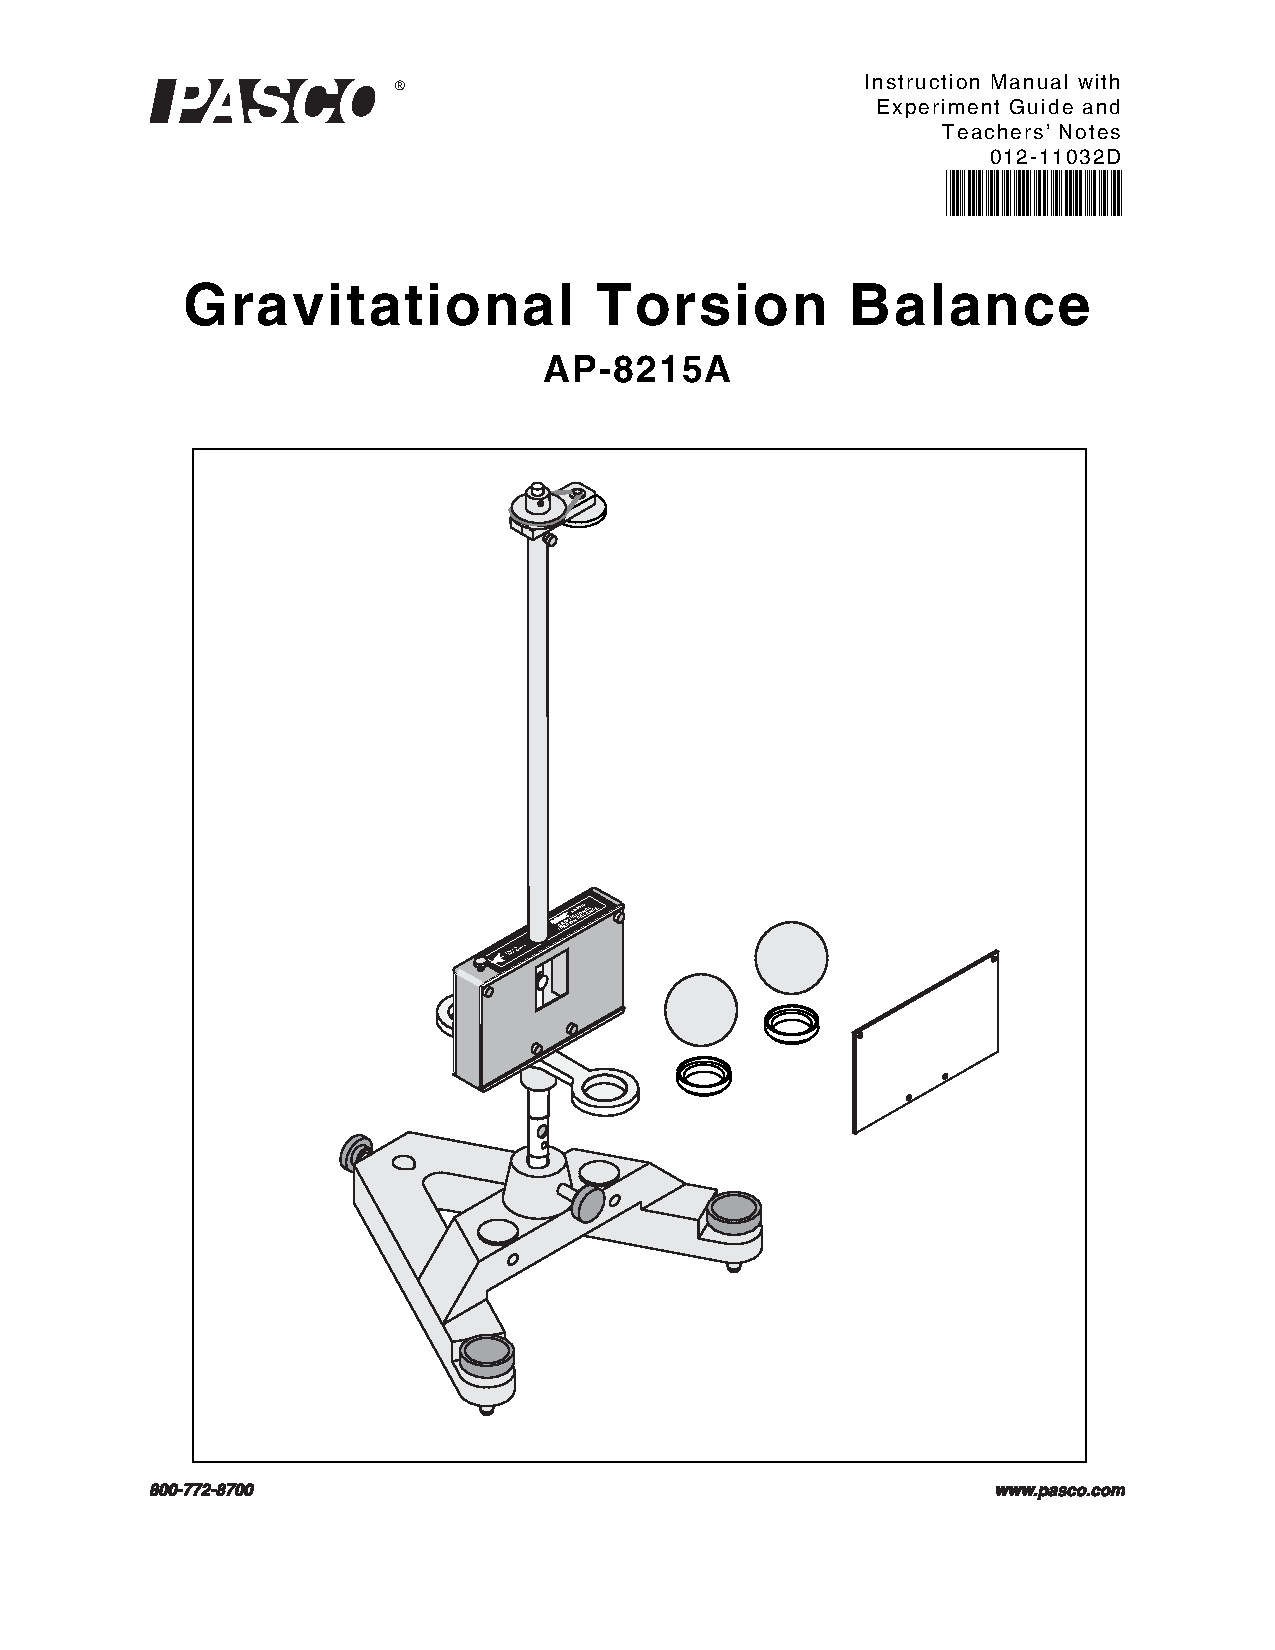
\includepdf[pages={1,3-8,16}]{pasco-cavendish/Gravitational-Torsion-Balance-Manual-AP-8215A.pdf}

% \bibliography{references,MyLibrary}
% \bibliographystyle{plain}
\printbibliography

\end{document}
